\documentclass[12pt,letterpaper]{article}
\usepackage{fontspec}
\usepackage[french]{babel}
\usepackage[margin=1in]{geometry}
\usepackage{amsmath,amssymb,amsthm}
\usepackage{graphicx,booktabs,multirow,array}
\usepackage{caption}
\usepackage{listings}
\usepackage{setspace}
\usepackage[hidelinks,hypertexnames=false]{hyperref}

\onehalfspacing
\graphicspath{{figures_fr/}}
\captionsetup{font=small,labelfont=bf}
\lstset{basicstyle=\ttfamily\scriptsize,breaklines=true,columns=fullflexible,
  keepspaces=true,upquote=true,showstringspaces=false}
\addto\captionsfrench{\renewcommand{\figurename}{Graphique}\renewcommand{\listfigurename}{Liste des graphiques}
  \renewcommand{\listtablename}{Liste des tableaux}\renewcommand{\tablename}{Tableau}}

% Les numéros des tableaux et graphiques suivent le mémoire déposé.
\newcommand{\numtable}[2]{\renewcommand{\thetable}{#1}\caption{#2}\addtocounter{table}{-1}}
\newcommand{\numfigure}[2]{\renewcommand{\thefigure}{#1}\caption{#2}\addtocounter{figure}{-1}}
\newcommand{\Et}{E_t}
\newcommand{\gbar}{\bar{g}}
\newcommand{\abar}{\bar{\alpha}}
\newcommand{\dtilde}{\tilde{\delta}}
\newcommand{\Theg}{\Theta_g}
\newcommand{\Thec}{\Theta_c}
\newcommand{\Thek}{\Theta_k}
\newcommand{\Thet}{\Theta_\tau}
\newcommand{\Phir}{\Phi_r}
\newcommand{\T}{\mathbb{T}}
\newcommand{\WW}{\mathcal{W}}
\newcommand{\TT}{\mathcal{T}}
\newcommand{\XX}{\mathcal{X}}
\newcommand{\DD}{\mathfrak{D}}
\newcommand{\pif}{\pi}


\begin{document}

\begin{titlepage}
\centering
{\large HEC MONTRÉAL\par}
\vspace{2cm}
{\LARGE\bfseries Dépenses publiques, mode de financement et multiplicateur budgétaire en trappe à liquidité\par}
\vspace{1cm}
par\par
\vspace{0.3cm}
{\large Aaron Israël\par}
\vspace{1.5cm}
Sciences de la gestion\par
(Option Économie Appliquée)\par
\vspace{1.5cm}
Mémoire présenté en vue de l’obtention du\par
grade de maîtrise ès sciences en gestion (M.Sc.)\par
\vspace{1.5cm}
Novembre 2023\par
\copyright{} Aaron Israël, 2023\par
\vfill
{\small \textbf{Version corrigée par l’auteur (2026).} Le mémoire déposé à HEC Montréal en 2023 reste la version officielle.\par}
\end{titlepage}

\pagenumbering{roman}
\setcounter{page}{3}

\section*{Résumé}
\addcontentsline{toc}{section}{Résumé}

Le but de ce mémoire est d’étudier la manière dont le mode de financement d’un plan de relance budgétaire affecte le multiplicateur des dépenses publiques dans différents contextes conjoncturels, soit en temps normal et en trappe à liquidité ; ce dernier scénario faisant référence à une situation dans laquelle le taux d’intérêt nominal est bloqué à son seuil minimal de zéro. Pour ce faire, nous développons un modèle dynamique d’équilibre général d’une économie fermée dans laquelle les dépenses publiques sont scindées en dépenses de fonctionnement (consommation) et d’investissement et sont financées soit par une taxe forfaitaire, soit par une taxe sur le revenu du travail, soit par dette.

Nous commençons par dériver des résultats analytiques dans une version stylisée du modèle, obtenue grâce à certaines hypothèses simplificatrices. En particulier, nous supposons que la durée de la trappe à liquidité est exogène et que le plan de relance (et l’augmentation de la taxe qui en résulte) prend fin dès que l’économie est sortie de trappe. Ce modèle indique que le multiplicateur budgétaire d’un plan de relance financé par une taxe sur le revenu du travail est plus grand que celui associé à un financement par taxe forfaitaire en trappe à liquidité. En simulant la version plus générale du modèle, cependant, nous montrons que lorsque le gouvernement a un budget équilibré en tout temps, le financement par taxe forfaitaire génère invariablement le multiplicateur le plus élevé, surtout lorsque le plan de relance est composé de dépenses de consommation. Ceci est dû au fait que l’effet inflationniste de la taxe sur le revenu perdure même lorsque l’économie est sortie de trappe. En revanche, lorsque le plan de relance est initialement financé par endettement public, le multiplicateur budgétaire est d’autant plus grand que la taxe sur le revenu du travail s’ajuste agressivement pour rembourser la dette, s’approchant ainsi du multiplicateur associé au financement par taxe forfaitaire.

\medskip
\noindent\textbf{Mots-clés :} Multiplicateur budgétaire, trappe à liquidité, équivalence ricardienne, politique monétaire, consommation publique, investissement public

\newpage
\tableofcontents
\newpage
\listoftables
\listoffigures

\section*{Note sur cette version}
\addcontentsline{toc}{section}{Note sur cette version}

Cette version reprend le contenu et la numérotation du mémoire déposé en 2023. Elle comporte des corrections mineures, dont aucune ne modifie les conclusions. Les graphiques ont été redessinés à partir d’une nouvelle exécution du modèle, selon la même disposition que l’original.

\section*{Remerciements}
\addcontentsline{toc}{section}{Remerciements}

Je tiens à remercier infiniment mon directeur de mémoire, Hafedh Bouakez, pour son soutien indéfectible tout au long de cette aventure académique. Ses conseils éclairés et son expertise pointue ont été d'une importance capitale dans la conception et la réalisation de ce mémoire.

En outre, je souhaite exprimer ma profonde reconnaissance envers ma famille. Vos encouragements m'ont donné la force de persévérer face aux défis et m'ont rappelé l'importance de poursuivre mes objectifs avec détermination.

\newpage
\pagenumbering{arabic}

\section{Introduction}

L’efficacité des dépenses publiques à stimuler l'activité économique a toujours été un sujet de débat important parmi les chercheurs et les décideurs politiques. Ce débat remonte en fait aux années 1930, lorsque l'économiste britannique John Maynard Keynes a développé sa théorie générale de l'emploi, de l'intérêt et de la monnaie.

Keynes a suggéré que dans les périodes de récession économique, l'État devrait intervenir pour stimuler l'activité économique en augmentant les dépenses publiques. Selon Keynes, cette politique aurait un effet multiplicateur sur l'économie car elle stimulerait la demande globale, ce qui à son tour créerait de l'emploi et stimulerait la croissance économique (Keynes 1936). Ainsi la politique budgétaire peut s’avérer être un outil redoutable quand la politique monétaire devient inefficace en période de récession dite classique, c’est-à-dire une croissance négative avec peu d’inflation voire de la déflation. On peut citer plusieurs grands plans de relance qui ont marqué l’histoire, comme le New Deal des années 1930 en réponse à la grande dépression, le plan Marshall en destination de l’Europe après la seconde guerre mondiale ou encore plus récemment les plans de relance pour lutter contre les effets négatifs de la pandémie COVID-19.

Ainsi, une vaste littérature scientifique s’est constituée pour tenter d’appréhender les facteurs d’influence des multiplicateurs autant d’un point de vue théorique qu’empirique. Dans ce mémoire, les principaux facteurs qui nous intéressent sont le contexte conjoncturel, particulièrement celui de la trappe à liquidité (i.e. lorsque le taux d’intérêt nominal est bloqué à son seuil minimal de 0), et le mode de financement des dépenses publiques lors d’un plan de relance budgétaire.

Notre étude est basée sur un modèle d’équilibre général dynamique et stochastique (DSGE) néo-Keynésien qui incorpore la concurrence monopolistique et la rigidité nominale des prix. Cette classe de modèles est considérée comme étant l’extension des modèles de cycle réel (RBC), dans lesquels la politique monétaire ne joue pas de rôle important puisque la monnaie y est neutre en tout temps. Notre modèle est celui d’une économie fermée dans laquelle les dépenses publiques sont scindées en dépenses de fonctionnement (consommation) et d’investissement et sont financées soit par une taxe forfaitaire, soit par une taxe sur le revenu du travail, soit par dette. Le modèle s’inspire des travaux de Bouakez, Guillard et Roulleau-Pasdeloup (2017, 2020), mais les étend en y introduisant une taxe distorsive sur le revenu du travail et l’endettement public.

La contribution de ce mémoire est d’évaluer les différences dans la taille du multiplicateur qui sont dues exclusivement aux différences dans le mode de financement du plan de relance budgétaire, et ce pour les dépenses de consommation et d’investissement publics. Pour ce faire, nous considérons divers scenarios qui partagent un état stationnaire commun, de sorte que seules les dépenses hors de l’état stationnaire sont financées différemment. Cet exercice contrefactuel a été très peu fait dans la littérature. Par ailleurs, le fait qu’il soit effectué dans le contexte d’un modèle ayant des fondements microéconomiques et où les anticipations sont rationnelles le rend immune à la critique de Lucas (Lucas, 1976).

Nous commençons par considérer une version stylisée de notre modèle, obtenue en imposant des hypothèses restrictives qui nous permettent de résoudre le modèle algébriquement (à une approximation de premier ordre près). En particulier, nous supposons que la durée de la trappe à liquidité est exogène et que le plan de relance (et l’augmentation de la taxe qui en résulte) prend fin dès que l’économie est sortie de trappe. Nous obtenons ainsi une expression algébrique pour le multiplicateur à la fois dans le cas d’un financement par taxe forfaitaire que dans celui d’un financement par taxe sur le revenu du travail. Nos résultats indiquent que bien que le multiplicateur soit plus élevé en temps normal dans le premier cas, ce résultat s’inverse lorsque l’économie est en trappe à liquidité; un financement par taxe sur le revenu du travail rendant le plan de relance encore plus expansionniste. Ceci est vrai quelle que soit la composition du plan de relance (en termes en dépenses de consommation et d’investissement).

L’intuition sous-jacente à ces prédictions réside dans le fait que la taxe sur le revenu du travail est inflationniste, puisqu’elle réduit l’offre de travail (d’où son caractère distorsif). En temps normal, cela amplifie l’augmentation du taux d’intérêt nominal et réel, réduisant ainsi l’effet sur la consommation et donc le multiplicateur budgétaire relativement au cas où le financement est effectué via un prélèvement forfaitaire. En trappe à liquidité, puisque le taux d’intérêt nominal est coincé à son seuil minimal de 0, l’effet inflationniste de la taxe distorsive réduit davantage la réponse du taux d’intérêt réel, amplifiant ainsi le multiplicateur. Ce mécanisme tient indépendamment du fait que le plan de relance est constitué de dépense de consommation ou d’investissement.

Par la suite, nous relâchons les hypothèses restrictives de la version simplifiée et considérons une version plus générale que nous résolvons de manière non-linéaire. Dans cette version, la sortie de trappe est endogène et l’effet inflationniste de la taxe sur le revenu du travail perdure même lorsque l’économie est sortie de trappe. Dans une économie où le gouvernement a un budget équilibré en tout temps, cela implique que le financement par taxe forfaitaire génère invariablement le multiplicateur le plus élevé en temps normal et en trappe. Ceci est d’autant plus vrai que le plan de relance est composé de dépenses de consommation. En revanche, lorsque le plan de relance est initialement financé par endettement public, plus la taxe sur le revenu du travail s’ajuste agressivement pour rembourser la dette, plus le multiplicateur est grand, s’approchant ainsi du multiplicateur associé au financement par taxe forfaitaire, surtout lorsque le plan de relance est composé de dépenses d’investissement et que le temps de construction du capital public est long. Le reste de ce mémoire est organisé comme suit : À la section 2, nous procédons à une revue de littérature qui traite des approches théoriques et empiriques existantes pour évaluer le multiplicateur budgétaire. La section 3 présente notre modèle théorique et la dérivation de ses conditions d’équilibre. À la section 4, nous présentons les résultats analytiques basés sur une version simplifiée du modèle. À la section 5, nous présentons les résultats basés sur la version générale du modèle avec et sans dette. La section 6 conclut.

\section{Revue de littérature}

\subsection{Approches théoriques}

Il existe une vaste littérature théorique portant sur les multiplicateurs de dépenses publiques en situation de trappe à liquidité. La plupart des études se sont cependant intéressées aux plans de relance budgétaire axés sur les dépenses de consommation et financés par une taxe forfaitaire.

Parmi les travaux les plus connus, on peut d’abord citer l’article de (Christiano, Eichenbaum et Rebelo, 2011) dans lequel les auteurs soutiennent que le multiplicateur budgétaire peut être bien supérieur à 1 lorsque le taux d'intérêt nominal est fixé à sa limite inférieure de zéro. Dans cette situation, les pressions inflationnistes qui résultent d’un plan de relance budgétaire entraînent une baisse du taux d’intérêt, de sorte que la hausse des dépenses publiques a un impact beaucoup plus important sur la production et l'emploi qu’elles ne l’auraient en temps normal. Pour étayer leur argumentation, les auteurs développent un modèle DSGE inspiré par Altig et al. (2011) dans lequel ils incluent un choc sur le facteur d’actualisation des ménages et sur les dépenses publiques.

Cette conclusion est corroborée par Eggertsson (2011) qui étudie les effets de réductions d'impôts et d’augmentations des dépenses publiques dans des circonstances économiques qui s’apparentent à celles ayant caractérisé la crise de 2008. Il trouve qu’en présence d’une politique monétaire très accommodante (maintenant le taux d’intérêt nominal à un niveau très faible), une réduction des impôts sur le travail et le capital contracte l’activité économique alors que l'augmentation temporaire des dépenses publiques a un effet expansionniste important, bien plus important que dans des circonstances normales.

Enfin, nous pouvons également citer l’article de Woodford (2011) qui décrit les facteurs clés qui déterminent la taille du multiplicateur budgétaire dans un modèle néo-Keynésien. Il démontre que la rigidité des prix ou des salaires permet d’obtenir des multiplicateurs plus importants que dans un modèle néoclassique, bien que la taille du multiplicateur dépende de manière cruciale de la réponse de la politique monétaire. Un multiplicateur bien supérieur à 1 est possible lorsque la politique monétaire est contrainte par la limite inférieure de zéro, et dans ce cas, le bien-être s’améliore si les dépenses publiques augmentent pour combler partiellement l'écart de production qui résulte de l'incapacité des autorités monétaires à abaisser les taux d'intérêt.

\subsubsection{Mode de financement des dépenses publiques}

Tel que mentionné ci-dessus, une grande partie de la littérature suppose que les dépenses publiques sont financées par une taxe forfaitaire en tout temps, même lors d’un plan de relance du gouvernement. Ainsi ce dernier a un budget équilibré à chaque période, ce qui implique que, dans le cadre d’un modèle macroéconomique d’équilibre général, la contrainte budgétaire du gouvernement n’est pas incluse dans les conditions d’équilibre. Lorsque les taxes forfaitaires sont les seuls prélèvements disponibles, l’hypothèse de budget équilibré n’est pas restreignante dans la mesure où l’équivalence ricardienne tient. Selon cette proposition – d’abord développée par David Ricardo au début du 19ème siècle et plus tard élaborée par Barro (1974) – le financement des dépenses publiques par des impôts forfaitaires actuels ou futurs aura des effets équivalents sur l'économie. Dans le deuxième cas, la hausse initiale des dépenses est alors financée par une hausse de la dette publique.

Cette approche peut s’avérer plus facilitante d’un point de vue pratique, mais est néanmoins peu réaliste : les taxes forfaitaires ne sont jamais utilisées pour financer les plans de relance. La contribution de ce mémoire est de considérer un financement alternatif basé sur l’impôt sur le revenu du travail, sans ou avec possibilité d’endettement public. Contrairement à la taxe forfaitaire, l’impôt sur le revenu du travail est distorsif. L’équivalence ricardienne ne tient donc pas dans ce cas.

Très peu d’études théoriques se sont intéressées aux effets des dépenses publiques en situation de trappe à liquidité en l’absence d’équivalence ricardienne. Nakata (2017) démontre qu’indépendamment du type d'impôt disponible et du niveau d'endettement initial, la politique budgétaire optimale en réponse à un choc adverse se caractérise par une augmentation des dépenses suivie d'une réduction en dessous de leur niveau initial et d'un éventuel retour à celui-ci. Cependant, l'ampleur des variations des dépenses publiques ainsi que leurs implications sur le bien-être dépendent fortement de l'instrument fiscal disponible et du niveau d'endettement initial.

Aloui et Eyquem (2019) étudient le lien entre l'ampleur de l'endettement public et l'efficacité des dépenses publiques à stimuler l’économie en temps normal et en trappe à liquidité. Ils développent un modèle néo-Keynésien dans lequel la trappe à liquidité est générée au moyen d’un choc sur la qualité du capital privé. Les dépenses du gouvernement sont financées par des taxes sur le revenu du travail, sur le revenu du capital et par de la dette. En temps normal, lorsque l’économie est caractérisée par une dette publique initiale élevée (en pourcentage du PIB), cela tend à réduire le multiplicateur budgétaire. En revanche, en situation de trappe à liquidité, des niveaux élevés de la dette publique produisent des multiplicateurs plus importants.

Lemoine et Lindé (2023), quant à eux, considèrent un large éventail d’instruments fiscaux dans un modèle non-Ricardien et montrent qu’en trappe à liquidité, les politiques fiscales conventionnelles (telles que les dépenses publiques en infrastructure) peuvent être plus efficaces que les politiques fiscales non conventionnelles (telles qu’une augmentation graduelle de la taxe sur les ventes jumelée à une réduction de l'impôt sur le revenu du travail). Cela est particulièrement vrai lorsque la crédibilité du gouvernement est faible, et que la trappe à liquidité est causée par des chocs non fondamentaux, ou lorsque les décideurs ont du mal à coordonner l'ajustement de la taxe de vente avec un changement substantiel de l'impôt sur le revenu du travail.

\subsubsection{Dépenses publiques de consommation et d'investissement en trappe à liquidité}

Les dépenses du gouvernement peuvent se décomposer en des dépenses de consommation (ou de fonctionnement) et d’investissement. Ces dernières servent à accroître le stock de capital public après un délai, souvent appelé ‘temps de construction’. L’un des premiers articles à introduire le capital public dans un modèle de cycle réel, sujet à une contrainte de temps de construction est Kydland et Prescott (1982). Les auteurs y démontrent que l’hypothèse couramment utilisée d’un temps de construction d’un seul trimestre est inadéquate pour expliquer les fluctuations cycliques des agrégats macroéconomiques aux États-Unis. Ils suggèrent qu’un temps de construction de plusieurs trimestres est nécessaire pour y parvenir. Une telle hypothèse a donc été reprise dans un grand nombre d’articles dont celui de Bouakez, Guillard et Roulleau-Pasdeloup (2017) qui nous servira de point de référence, notamment dans la construction du modèle et dans la résolution analytique.

Dans ce travail, les auteurs étudient l’efficacité des dépenses en investissement public comme un outil de relance dans une économie néo-Keynésienne où une fraction des dépenses publiques augmente le stock de capital public, lui-même sujet à une contrainte de temps de construction. Ils mettent alors en évidence l’importance de décomposer les dépenses du gouvernement en ses composantes de consommation et d’investissement. En particulier, ils démontrent que ne pas tenir compte de la composition d’un plan de relance en négligeant sa composante investissement conduirait à sous-estimer significativement le multiplicateur, surtout en trappe à liquidité.

Boehm (2020) explique également l’importance quant à la taille du multiplicateur de la manière dont sont allouées les dépenses publiques. Le modèle qu’il développe prédit qu’en temps normal, le multiplicateur associé aux dépenses publiques en investissement est plus petit que celui associé à la consommation publique, et ce lorsque les variations de dépenses sont de courte durée. Deux explications équivalentes sont proposées pour ce résultat. La première souligne que les chocs de dépenses d'investissement n'ont pratiquement aucun effet sur l'offre de travail des ménages, c'est-à-dire qu'ils n'incitent pas les ménages à travailler davantage. La deuxième explication met en avant le fait qu’en raison d'une plus grande substituabilité intertemporelle, l'investissement privé diminue davantage après les chocs de dépenses publiques d'investissement que la consommation privée après les chocs de dépenses publiques de consommation.

Dans le même esprit, Ramey (2020) étudie les effets à court et à long terme de l'investissement public sur l'économie. L'analyse théorique considère à la fois les modèles néoclassiques et néo-Keynésiens. Les multiplicateurs à long terme de l'investissement public dépendent essentiellement de l'élasticité de la fonction de production par rapport au capital public et de la situation initiale de l'économie par rapport au niveau socialement optimal du capital public. Partir d’un niveau de capital bas avec une élasticité élevée permet d’obtenir des multiplicateurs élevés. En outre, l’auteure constate que bien que l'investissement public ait des effets significatifs à long terme, les multiplicateurs à court terme sont généralement inférieurs à ceux de la consommation publique en temps normal, en raison des retards de construction et de la propension de l'investissement public à évincer l’investissement privé. L’auteure mentionne, cependant, qu'il existe un soutien à la fois théorique et empirique à l’idée que le multiplicateur à court terme de l'investissement public soit plus élevé lorsque les taux d'intérêt sont à la limite inférieure zéro. Les mécanismes théoriques qui conduisent à cet effet impliquent que le financement des dépenses publiques par des impôts sur le revenu, plutôt que par des déficits, conduit à des multiplicateurs plus élevés.

Finalement, Bouakez, Guillard et Roulleau-Pasdeloup (2020) s’intéressent à la politique fiscale optimale dans une économie plongée dans une récession profonde caractérisée par une trappe à liquidité et où le gouvernement peut allouer ses dépenses à la consommation et à l'investissement public, ce dernier augmentant le stock de capital public sous une contrainte de temps de construction. Les résultats de l'étude suggèrent que la réponse optimale à un tel choc consiste à accroitre les dépenses publiques et en modifier la composition en augmentant la part des dépenses d’investissement.

\subsection{Approches empiriques}

Il existe aussi une très vaste littérature qui se propose d’estimer empiriquement les multiplicateurs budgétaires. L’abondance des travaux existants rend, cependant, impossible la tâche d’en faire une revue exhaustive dans un espace restreint. Ramey (2019) examine l'état des connaissances récentes sur le sujet en se basant sur des estimations empiriques effectuées dans la décennie ayant suivi la crise de 2008. Les estimations recensées se situent principalement dans une fourchette étroite allant de 0,6 à 1. Cependant, cette fourchette s'élargit lorsque l'on prend en compte des caractéristiques nationales spécifiques, telles que le régime de change et le type de dépenses gouvernementales. Ainsi, dans les prochaines sous-sections, nous présentons les articles les plus influents et qui se rapprochent le plus des préoccupations de ce mémoire.

\subsubsection{Estimation du multiplicateur par type de dépenses publiques}

Perotti (2004) fut le premier à utiliser un VAR structurel afin de comparer les effets macroéconomiques des trois principales catégories des dépenses gouvernementales : l'investissement, la consommation et les transferts aux ménages, tant en termes de la taille que de la rapidité de leurs effets sur le PIB et ses composantes. Les chocs de dépenses sont identifiés via une décomposition Cholesky de la matrice de variance-covariance des résidus statistiques. Ses résultats ne permettent pas de conclure que les chocs d'investissement public sont plus efficaces que les chocs de consommation publique pour stimuler le PIB. Ceci est vrai à la fois à court terme et, de manière peut-être plus surprenante, à long terme. En fait, l'investissement gouvernemental semble décourager l'investissement privé, en particulier dans le logement et les machines et équipements.

Bouakez, Larocque et Normandin (2018) entreprennent une analyse désagrégée des effets des dépenses gouvernementales sur l’activité économique aux États-Unis, en décomposant la consommation et l’investissement public en diverses sous-catégories. Pour chaque sous-catégorie, les auteurs estiment un vecteur autorégressif structurel au sein duquel les chocs de dépenses publiques sont identifiés en exploitant l’hétéroscédasticité conditionnelle des perturbations structurelles, ce qui permet de relâcher les restrictions d’identification communément utilisées dans la littérature. Les catégories de dépenses qui permettent d’obtenir les multiplicateurs les plus grands (et qui sont supérieurs à 1) sont les achats de biens durables et les investissements en structures. Les résultats suggèrent également qu’il y a peu de rapport entre l’importance d’une catégorie de dépenses publiques et l’ampleur de son effet sur la production agrégée.

Boehm (2020) compare également les multiplicateurs associés à la consommation et à l’investissement public en utilisant des données de panel de l’OCDE allant de 2003 à 2016. Sa méthodologie est basée sur les projections locales de Jordà (2005) et les multiplicateurs sont obtenus en s’inspirant de l’approche de Ramey et Zubairy (2018). Les résultats empiriques soutiennent largement les prédictions de son modèle théorique. Premièrement, le multiplicateur associé aux dépenses publiques en investissement est plus petit que celui associé aux dépenses publiques en consommation. Deuxièmement, la différence entre ces deux multiplicateurs est due à un effet d’éviction important sur l'investissement privé, causé par une hausse du taux d'intérêt réel propre au secteur des biens d'investissement.

\subsubsection{Estimation du multiplicateur en conditionnant sur le cycle économique}

Certains travaux empiriques ont estimé le multiplicateur en prenant en compte l’aspect conjoncturel de l’économie. Ils se proposent de déterminer si le multiplicateur budgétaire varie selon que l’économie est en récession ou en expansion. On peut citer l’étude d’Auerbach et Gorodnichenko (2012) qui utilisent un modèle économétrique à changement de régime pour évaluer le multiplicateur en récession et en expansion en utilisant des données américaines. Ils constatent de grandes différences dans la taille des multiplicateurs de dépenses dans ces deux phases du cycle, la politique budgétaire étant considérablement plus efficace durant les récessions. Plus spécifiquement, les auteurs obtiennent un multiplicateur entre 0 et 0,5 en expansion, et entre 1 et 1,5 en récession.

De la même manière, Ramey et Zubairy (2018) tentent de déterminer si le multiplicateur budgétaire est plus élevé pendant les périodes de ralentissement économique ou lorsque les taux d'intérêt nominaux sont proches de la limite inférieure zéro. À l'aide de nouvelles données historiques trimestrielles américaines couvrant plusieurs grandes guerres et récessions profondes, les auteures estiment des multiplicateurs positifs, mais inférieurs à 1, quel que soit le niveau de ralentissement de l'économie. Ces résultats sont robustes à deux principaux schémas d'identification, à deux méthodologies d'estimation différentes et à de nombreuses spécifications alternatives. En revanche, les résultats sont plus mitigés pour la limite inférieure zéro du taux d’intérêt, avec des spécifications impliquant des multiplicateurs aussi élevés que 1,5. Les auteures procèdent également à une comparaison de la méthode de Jordà (2005) et celle utilisée par Auerbach et Gorodnichenko (2012) citée précédemment. Elles montrent alors que les résultats d’Auerbach et Gorodnichenko (2012) dépendent d'une hypothèse simplificatrice qui n'est pas une bonne approximation pour leur échantillon. Elles concluent ainsi que leurs estimations des multiplicateurs en récession sont beaucoup plus faibles une fois cette hypothèse relâchée. Un autre article empirique qui prend en compte le cycle économique et en particulier la trappe à liquidité est celui de Miyamoto, Nguyen et Sergeyev (2018). Les auteurs utilisent des données trimestrielles japonaises de 1980 à 2014 pour estimer les effets des chocs de dépenses publiques sur l'économie lorsque le taux d'intérêt nominal se situe à sa limite inférieure zéro et également en temps normal. Plusieurs facteurs font de l'expérience japonaise le meilleur cas pour étudier les effets des dépenses gouvernementales en trappe à liquidité. Premièrement, le Japon a connu la plus longue période de trappe, avec un taux d'intérêt nominal proche de zéro depuis 1995. Deuxièmement, pendant cette période, le Japon a traversé quatre cycles économiques, ce qui permet de différentier les effets issus des périodes de trappe et ceux venant des périodes de récession. Le multiplicateur à l’impact estimé par les auteurs est de 1,5 pendant la période de trappe, alors qu’il est de 0,6 en temps normal. Les dépenses publiques stimulent la consommation et l’investissement privé en trappe à liquidité, mais les évincent pendant les périodes hors trappe. Les auteurs concluent que certaines des conclusions empiriques sont cohérentes avec le mécanisme néo-Keynésien.

\section{Modèle}

Le modèle que nous présentons dans cette section permet de calculer le multiplicateur budgétaire avec différents types de financement dans le contexte d’une économie fermée. Nous voulons évaluer dans quelle mesure la présence d’un financement par taxe distorsive d’un plan de relance influence le multiplicateur en temps normal et en trappe à liquidité comparativement à un financement par taxe forfaitaire.

Ce modèle est basé sur les travaux de Bouakez, Guillard et Roulleau-Pasdeloup (2017, 2020), notamment pour la manière de générer une trappe à liquidité. Dans Bouakez, Guillard et Roulleau-Pasdeloup (2017), la trappe à liquidité est générée par un choc sur le facteur d’escompte psychologique des ménages, alors que dans Bouakez, Guillard et Roulleau-Pasdeloup (2020), elle résulte d’un choc affectant la préférence pour la liquidité.

L’économie est composée d’une infinité de ménages identiques et d’un continuum de firmes en concurrence monopolistique produisant des biens intermédiaires différenciés et indexés par $i \in [0,1]$. Ces biens servent à produire un bien final homogène. Le modèle contient du capital public qui sert d’intrant dans la production des biens différenciés. Le capital public est sujet à une contrainte de temps de construction.

\subsection{Ménages}

L’économie est composée d’une infinité de ménages identiques. Le ménage représentatif a la fonction d’utilité intertemporelle suivante :
\begin{equation}
\Et \sum_{s=0}^{\infty} \prod_{x=0}^{s} \beta_x \left[ U(C_{t+s}, N_{t+s}) + \zeta_{t+s} F\!\left(\frac{B_{t+s}}{P_{t+s}}\right) \right] \tag{1}
\end{equation}
où $C_t$ est la consommation, $N_t$ le nombre d’heures travaillées et $\beta_x$ le facteur d’actualisation stochastique du ménage compris entre 0 et 1, vérifiant $\beta_0 = 1$. La fonction d’utilité est la suivante :
\begin{align}
U_t &= \frac{\left(C_t^{\gamma}(1-N_t)^{1-\gamma}\right)^{1-\sigma}}{1-\sigma} \quad \text{si } \sigma \neq 1 \tag{2}\\
U_t &= \gamma \ln C_t + (1-\gamma)\ln(1-N_t) \quad \text{si } \sigma = 1 \tag{3}
\end{align}
$B_t$ est le nombre d’unités de l’actif sans risque, soit les obligations gouvernementales, $P_t$ est le prix du bien final, et $F$ est une fonction croissante et concave et est telle que $F(0)=0$ et $F'(0)=1$. L’hypothèse selon laquelle la fonction d’utilité dépend positivement de la valeur réelle de la quantité d’actifs sans risque reflète la préférence du ménage pour la liquidité et la sécurité de ces actifs. $\zeta_t$ est une variable exogène qui suit le processus autorégressif d’ordre 1 suivant :
\begin{equation}
\zeta_t = \rho_\zeta \zeta_{t-1} + \epsilon_{\zeta_t} \tag{4}
\end{equation}
où $0 < \rho_\zeta < 1$ est le coefficient d’autocorrélation de premier ordre de $\zeta_t$ et $\epsilon_{\zeta_t}$ suit une loi normale centrée sur zéro avec un écart type $\sigma_\zeta$. Ainsi, une trappe à liquidité peut être générée en introduisant un choc positif $\epsilon_{\zeta_t}$ ; ce choc ayant pour effet d’augmenter l’épargne des ménages dans les actifs sans risque et donc de faire baisser le taux d’intérêt nominal. Lorsque le choc est suffisamment important, ce dernier diminue jusqu’à ce qu’il atteigne sa borne inférieure de zéro.

Le ménage représentatif entame la période $t$ avec $B_{t-1}$ unités d’obligations à échéance d’une période. Pendant cette période, le ménage reçoit un revenu $\WW_t N_t$ issu de son travail sur lequel il paie un impôt $\tau_t$ au gouvernement et un dividende, $\DD_t$, versé par les entreprises monopolistiques. Les revenus du ménage sont alloués à la consommation, à l’achat d’un nouveau stock d’obligations, $B_t$, et au paiement d’une taxe forfaitaire $\TT_t$. La contrainte budgétaire du ménage est la suivante :
\begin{equation}
P_t C_t + \frac{B_t}{1+i_t} + \TT_t \leq (1-\tau_t)(\WW_t N_t) + B_{t-1} + \DD_t \tag{5}
\end{equation}
où le côté gauche de l’équation représente les dépenses du ménage et le côté droit ses revenus. $\WW_t$ est le salaire nominal, $\frac{1}{1+i_t}$ est le prix d’une obligation gouvernementale sans risque au temps $t$.

Le ménage maximise (1) sujet à la contrainte (5) et à une condition d’absence de jeu de Ponzi. Les conditions de premier ordre peuvent être résumées de la manière suivante :
\begin{align}
W_t &= \frac{-U_{N_t}}{U_{C_t}(1-\tau_t)} \tag{6}\\
U_{C_t} &= \zeta_t F'\!\left(\frac{B_t}{P_t}\right) + (1+i_t)\Et \beta_{t+1} \frac{U_{C_{t+1}}}{1+\pi_{t+1}} \tag{7}
\end{align}
où $W_t = \frac{\WW_t}{P_t}$ est le salaire réel du ménage, $U_{C_t}$ est la dérivée de la fonction d’utilité par rapport à $C_t$, $F'(.)$ est la dérivée de la fonction $F$ par rapport à $\frac{B_t}{P_t}$ et $\pi_t = \left(\frac{P_t}{P_{t-1}}\right) - 1$ est le taux d’inflation entre $t-1$ et $t$. Ainsi (6) représente l’équation d’offre de travail et (7) l’équation d’Euler.

\subsection{Firmes}

Le bien final est produit par des entreprises en concurrence pure et parfaite en utilisant la technologie suivante :
\begin{equation}
Y_t = \left[\int_0^1 Y_t(i)^{\frac{\theta-1}{\theta}}\, \mathrm{d}i\right]^{\frac{\theta}{\theta-1}} \tag{8}
\end{equation}
où $Y_t(i)$ est la quantité de bien intermédiaire $i$ et $\theta \geq 1$ est l’élasticité de substitution entre les biens intermédiaires. La demande pour le bien intermédiaire $i$ est donnée par :
\begin{equation}
Y_t(i) = \left(\frac{P_t(i)}{P_t}\right)^{-\theta} Y_t \tag{9}
\end{equation}
où $P_t(i)$ est le prix du bien intermédiaire $i$.

Les firmes produisant les biens intermédiaires œuvrent dans un contexte de concurrence monopolistique et utilisent la main-d’œuvre et le capital public comme intrants :
\begin{equation}
Y_t(i) = F(N_t(i), K_t) = N_t^a K_t^b \tag{10}
\end{equation}
où $a$ et $b$ sont respectivement l’élasticité de la production par rapport au travail et au capital public ; elles sont supérieures ou égales à zéro. Les producteurs de biens intermédiaires sont assujettis à un coût d’ajustement des prix à la Rotemberg :
\begin{equation}
\Xi_t(i) = \frac{\XX}{2}\left(\frac{P_t(i)}{P_{t-1}(i)} - 1\right)^2 Y_t \tag{11}
\end{equation}
où $\XX \geq 0$ gouverne la magnitude du coût d’ajustement. Le dividende réel, $D_t(i) = \DD_t(i)$, payé par la firme $i$ est donné par :
\begin{equation}
D_t(i) = \frac{P_t(i)}{P_t} Y_t(i) - W_t N_t(i) - \Xi_t(i) \tag{12}
\end{equation}
Cette firme choisit $P_t(i)$ et $N_t(i)$ pour maximiser sa valeur de marché :
\begin{equation}
\Et \sum_{s=0}^{\infty} \prod_{x=0}^{s} \beta_x \frac{U_{c,t+s}}{U_{c,t}} \DD_{t+s}(i) \tag{13}
\end{equation}
sous les contraintes données par la fonction de production (10) et la fonction de demande (9). Étant donné que toutes les entreprises sont symétriques, les conditions de premier ordre sont données par :
\begin{align}
MC_t &= \frac{\theta-1}{\theta} + \frac{\XX}{\theta}\pi_t(1+\pi_t) - \frac{\XX\beta_t}{\theta}\Et\frac{U_{c,t+1}}{U_{c,t}}\frac{Y_{t+1}}{Y_t}\pi_{t+1}(1+\pi_{t+1}) \tag{14}\\
MC_t &= \frac{W_t}{F_{N_t}} \tag{15}
\end{align}
où $MC_t$ est le coût marginal réel.

\subsection{Autorités monétaires et fiscales}

Le gouvernement finance ses dépenses, $G_t$, par de la dette, l’impôt sur le revenu du travail $\tau_t$ et la taxe forfaitaire. La contrainte budgétaire peut se décliner de la manière suivante :
\begin{equation}
P_t G_t + i_t B_{t-1} \leq \TT_t + \tau_t \WW_t N_t + B_t - B_{t-1} \tag{16}
\end{equation}
Dans nos analyses, nous considérerons un cas avec dette et un autre sans dette. Dans le cas sans dette, nous considérerons $B_t$ nul en tout temps et supposons que la taxe forfaitaire réelle, $T_t = \frac{\TT_t}{P_t}$, est telle que :
\begin{equation}
T_t = \eta G_t + (1-\eta)T \tag{17}
\end{equation}
où $G$ et $T$ sont respectivement les dépenses publiques et la taxe forfaitaire à l’état stationnaire. Ainsi, si nous fixons $\eta = 1$, les dépenses publiques sont financées en tout temps (à l’état stationnaire et hors de l’état stationnaire) par la taxe forfaitaire $T_t$ qui s’ajuste à chaque période pour avoir un budget équilibré. Notons que dans ce cas, $\tau_t = 0$ et l’équivalence ricardienne tient. En revanche, si nous fixons $\eta = 0$, la taxe forfaitaire est égale à son niveau stationnaire en tout temps et la taxe sur le revenu du travail est non nulle hors de l’état stationnaire du modèle, c’est-à-dire lors d’un choc des dépenses publiques. Cette modélisation nous permet d’isoler les effets sur les multiplicateurs des différences dans le type de financement des plans de relance puisque l’état stationnaire est invariable.

Lorsque le gouvernement finance (initialement) ses dépenses par dette, nous devons spécifier la manière dont l’impôt sur le revenu s’ajuste pour éventuellement permettre au gouvernement de rembourser sa dette. Nous considérons alors le processus suivant :
\begin{equation}
\tau_t = (1-\rho_n)\tau + \rho_n \tau_{t-1} + (1-\rho_n)\gamma_n\left(\frac{B_{t-1}}{Y_t} - \frac{B}{Y}\right) \tag{18}
\end{equation}
où $\tau$ et $\frac{B}{Y}$ sont, respectivement, le niveau de la taxe sur le revenu du travail et le ratio dette/PIB à l’état stationnaire, $\rho_n$ est le coefficient d’autocorrélation de premier ordre de la taxe et $\gamma_n$ l’élasticité de la taxe sur le revenu du travail par rapport au niveau de dette.

Les dépenses en investissement public augmentent le stock du capital en suivant la loi d’accumulation suivante :
\begin{equation}
K_t = (1-\delta)K_{t-1} + G^i_{t-\T} \tag{19}
\end{equation}
où $\T$ est le nombre de trimestres nécessaires à la construction du capital public comme proposé par Kydland et Prescott (1982). Nous considérons ainsi différents temps de construction, notamment 1 et 16 trimestres.

Les dépenses publiques en investissement suivent le processus suivant :
\begin{equation}
G^i_t = G^i + \alpha(G_t - G) \tag{20}
\end{equation}
où $\alpha$ est la part allouée à l’investissement dans les dépenses publiques lors d’un plan de relance. Les dépenses publiques sont déterminées par un processus autorégressif :
\begin{equation}
\frac{G_t - G}{Y} = \rho\left(\frac{G_{t-1} - G}{Y}\right) + \epsilon_g \tag{21}
\end{equation}
où $0 \leq \rho \leq 1$, $Y$ est le PIB à l’état stationnaire et $\epsilon_g$ est un bruit blanc qui représente le choc sur les dépenses publiques.

Les autorités monétaires suivent une règle de Taylor avec une contrainte de non-négativité sur le taux d’intérêt nominal. La règle prend en compte le taux d’intérêt passé, l’inflation et l’écart du PIB par rapport à son état stationnaire. Elle est donnée par :
\begin{equation}
i_t = \max\left(0, (1+r_\beta)\left(\frac{1+i_{t-1}}{1+r_\beta}\right)^{\rho_r}\left[\left(\frac{1+\pi_t}{1+\pi}\right)^{\phi_\pi}\left(\frac{Y_t}{Y}\right)^{\phi_y}\right]^{1-\rho_r} - 1\right) \tag{22}
\end{equation}
où $r_\beta = \beta^{-1} - 1$, $\beta$ étant la valeur de $\beta_s$ à l’état stationnaire, $0 < \rho_r < 1$, $\phi_\pi > 1$ et $\phi_y > 0$.

À noter également que la contrainte des ressources de ce modèle prend en compte les coûts d’ajustement des prix. On a donc :
\begin{equation}
Y_t = C_t + G_t + \frac{\XX}{2}\pi_t^2 Y_t \tag{23}
\end{equation}

\section{Résultats analytiques dans un modèle simplifié}

Dans cette section, nous considérons une version suffisamment simplifiée du modèle décrit ci-dessus pour nous permettre de dériver des solutions analytiques caractérisant le multiplicateur budgétaire en temps normal et en trappe à liquidité pour les cas avec et sans financement distorsif du plan de relance. Pour ce faire, nous supposons que la dette publique est nulle en tout temps, que le temps de construction du capital public est nul ($\T = 0$), que la dépréciation du capital est complète après un trimestre ($\delta = 1$), que la règle de Taylor est telle que $\rho_r = \phi_y = 0$, et que la fonction d’utilité du ménage est additivement séparable entre la consommation et le travail ($\sigma = 1$). Nous faisons également abstraction du choc sur la préférence pour la liquidité ($\zeta_t$ est nul en tout temps) et supposons plutôt que le facteur d’escompte suit un processus markovien à deux états.

\subsection{Modèle linéarisé}

On résout le modèle en linéarisant les équations autour d’un état stationnaire ayant une inflation nulle. Dans ce qui suit, les variables sans indice de temps indiquent qu’elles sont à l’état stationnaire et les variables en minuscules indiquent leur déviation en pourcent par rapport à leur valeur stationnaire. Par exemple $x_t = \frac{X_t - X}{X}$ sauf pour $g_t = \frac{G_t - G}{Y}$. Le modèle linéarisé est donc le suivant :
\begin{align}
y_t &= (1-\gbar)c_t + g_t \tag{24}\\
n_t &= \frac{F}{F_N N}y_t - \frac{F_K K}{F_N N}k_t \tag{25}\\
c_t &= \Et c_{t+1} + \frac{U_C}{U_{CC}C}\left(i_t - \Et\pi_{t+1} - r_{\beta,t}\right) \tag{26}\\
w_t &= \left(\frac{U_{CN}C}{U_C} - \frac{U_{CC}C}{U_C}\right)c_t + \left(\frac{U_{NN}N}{U_N} - \frac{U_{CN}N}{U_C}\right)n_t + \tau_t \tag{27}\\
\tau_t &= \frac{g_t}{a} \tag{28}\\
\pi_t &= \beta\Et\pi_{t+1} + \kappa\, mc_t \tag{29}\\
mc_t &= w_t - \frac{F_{NN}N}{F_N}n_t - \frac{F_{NK}K}{F_N}k_t \tag{30}\\
k_t &= \alpha\dtilde g_t \tag{31}\\
i_t &= \max(0; r_\beta + \phi_\pi\pi_t) \tag{32}
\end{align}
où $\kappa = \frac{\theta-1}{\XX}$ ; $\dtilde = \frac{\delta}{\abar\gbar}$ ; $\gbar = \frac{G}{Y}$ ; $r_{\beta,t} = \frac{1}{\beta_t} - 1$ et où $\abar$ représente la part des dépenses gouvernementales allouée à l’investissement, soit $\frac{G^i}{G}$. Lorsque le plan de relance est financé par une taxe forfaitaire, $\tau_t$ est égal à zéro en tout temps.

\subsection{Le multiplicateur budgétaire en temps normal}

En réarrangeant le système d’équations qui vient d’être décrit et en considérant $r_{\beta,t}$ comme constant, on peut le présenter par deux équations représentant la demande et l’offre agrégées :
\begin{align}
c_t &= \Et c_{t+1} - \Phir(\phi_\pi\pi_t - \Et\pi_{t+1}) \tag{33}\\
\pi_t &= \beta\Et\pi_{t+1} + \kappa\left(\Thec c_t + (\Theg + \Thet - \alpha\dtilde\Thek)g_t\right) \tag{34}
\end{align}
où
\begin{align}
\Phir &= -\frac{U_C}{U_{CC}C} \tag{35}\\
\Theg &= \left(\frac{U_{NN}N}{U_N} - \frac{U_{CN}N}{U_C} + \frac{F_{NN}N}{F_N}\right)\frac{F}{F_N N} \tag{36}\\
\Thec &= \Phir^{-1} + (1-\gbar)\Theg \tag{37}\\
\Thek &= \frac{F_{NK}K}{F_N} + \frac{F_K K}{F}\Theg \tag{38}\\
\Thet &= \frac{1}{a} \quad \text{dans le cas du financement par taxe sur le revenu du travail} \tag{39}\\
\Thet &= 0 \quad \text{dans le cas du financement par taxe forfaitaire} \tag{40}
\end{align}
Puisque cette version du modèle n’a pas de variables d’état, nous avons $\Et\pi_{t+1} = \rho\pi_t$ et $\Et c_{t+1} = \rho c_t$. En combinant (33) et (34), on peut exprimer $c_t$ en fonction de $g_t$ :
\begin{equation}
c_t = \Omega g_t \tag{41}
\end{equation}
où
\begin{equation}
\Omega = \frac{-\Phir(\phi_\pi-\rho)\kappa\left(\Theg + \Thet - \alpha\dtilde\Thek\right)}{(1-\rho)(1-\beta\rho) + \Phir(\phi_\pi-\rho)\kappa\Thec} \tag{42}
\end{equation}
En utilisant $y_t = (1-\gbar)c_t + g_t$, on peut obtenir une solution analytique pour le multiplicateur, $m = dY_t/dG_t = y_t/g_t$ :
\begin{equation}
m = 1 + (1-\gbar)\Omega \tag{43}
\end{equation}
Avec du réarrangement algébrique et en utilisant le fait que $\Thec = \Phir^{-1} + (1-\gbar)\Theg$, on démontre que la solution analytique du multiplicateur avec financement distorsif est la suivante :
\begin{equation}
m^d = \frac{1 + \Psi + (1-\gbar)\Phir\left(\alpha\dtilde\Thek - \Thet\right)}{1 + \Psi + (1-\gbar)\Phir\Theg} \tag{44}
\end{equation}
où $\Psi = \frac{(1-\rho)(1-\beta\rho)}{\kappa(\phi_\pi-\rho)} \geq 0$ mesure indirectement la rigidité des prix à travers le paramètre $\kappa$. Plus $\kappa$ est grand, plus les prix sont flexibles.

Étant donné que dans un contexte de financement par taxe forfaitaire $\Thet = 0$, le multiplicateur est donné par :
\begin{equation}
m^f = \frac{1 + \Psi + (1-\gbar)\Phir\alpha\dtilde\Thek}{1 + \Psi + (1-\gbar)\Phir\Theg} \tag{45}
\end{equation}
La proposition 1 ci-dessous établit que ce dernier est toujours supérieur à celui correspondant au financement par taxe sur le revenu du travail.

\medskip
\noindent\textbf{\emph{Proposition 1 :}}
\begin{equation}
m^d < m^f \tag{46}
\end{equation}
\noindent\textbf{\emph{Preuve :}} Étant donné que $\Thet$ est strictement supérieur à zéro, on peut affirmer qu’en temps normal le multiplicateur est plus élevé quand le plan de relance est financé par une taxe forfaitaire.

\subsection{Le multiplicateur budgétaire en trappe à liquidité}

Intéressons-nous maintenant au cas de la trappe à liquidité. Cette dernière survient quand les agents économiques augmentent suffisamment leur épargne, poussant alors le taux d’intérêt nominal vers le bas jusqu’à atteindre zéro. Ainsi, dans un premier temps, nous imposons un choc positif sur le facteur d’actualisation stochastique des ménages. Ce dernier suit donc le processus markovien suivant :
\begin{align}
\Pr[\beta_{t+1} = \beta^l \mid \beta_t = \beta^l] &= p \nonumber\\
\Pr[\beta_{t+1} = \beta^l \mid \beta_t = \beta] &= 0 \tag{47}
\end{align}
où $p$ est la probabilité que le facteur d’actualisation reste élevé à un niveau tel que $i_t$ est égal à zéro. On peut alors substituer $i_t$ dans l’équation (26) pour représenter le contexte de trappe à liquidité.
\begin{align}
c^l_t &= \Et c_{t+1} + \Phir\Et\pi_{t+1} \tag{48}\\
\pi^l_t &= \beta\Et\pi_{t+1} + \kappa\left(\Thec c^l_t + (\Theg + \Thet - \alpha\dtilde\Thek)g^l_t\right) \tag{49}
\end{align}
De la même manière qu’en temps normal, on peut exprimer $c^l_t$ en fonction de $g^l_t$ :
\begin{equation}
c^l_t = \Omega^l g^l_t \tag{50}
\end{equation}
où
\begin{equation}
\Omega^l = \frac{\Phir p\kappa\left(\Theg + \Thet - \alpha\dtilde\Thek\right)}{(1-p)(1-\beta p) - \Phir p\kappa\Thec} \tag{51}
\end{equation}
Le multiplicateur en trappe à liquidité est donc donné par :
\begin{equation}
m^{ld} = \frac{\Psi^l - 1 - (1-\gbar)\Phir\left(\alpha\dtilde\Thek - \Thet\right)}{\Psi^l - 1 - (1-\gbar)\Phir\Theg} \tag{52}
\end{equation}
où $\Psi^l = \frac{(1-p)(1-\beta p)}{\kappa p} > 0$.

Le multiplicateur correspondant au financement par taxe forfaitaire est obtenu en imposant $\Thet = 0$ :
\begin{equation}
m^{lf} = \frac{\Psi^l - 1 - (1-\gbar)\Phir\alpha\dtilde\Thek}{\Psi^l - 1 - (1-\gbar)\Phir\Theg} \tag{53}
\end{equation}
La proposition 2 ci-dessous établit que ce dernier est toujours inférieur à celui obtenu dans le cas d’un financement par taxe sur le revenu du travail.

\medskip
\noindent\textbf{\emph{Proposition 2 :}}
\begin{equation}
m^{ld} > m^{lf} \tag{54}
\end{equation}
\noindent\textbf{\emph{Preuve :}} De la même manière qu’en temps normal, $\Thet$ est strictement supérieur à zéro, alors en trappe à liquidité le multiplicateur est plus faible quand le plan de relance est financé par une taxe forfaitaire.

\medskip
Ainsi, un financement par taxe sur le revenu du travail produit des multiplicateurs qui sont inférieurs à ceux d’un financement forfaitaire en temps normal, mais supérieurs en trappe à liquidité. En temps normal, la taxe sur le revenu du travail est inflationniste, alors le taux d’intérêt nominal augmente plus que lorsqu’une telle taxe n’est pas en vigueur. Ainsi, à la suite de la hausse des dépenses publiques, le taux d’intérêt réel augmente plus dans le cas du financement par taxe sur le revenu du travail, ce qui atténue le multiplicateur. En trappe à liquidité, le taux nominal est bloqué à zéro, alors le taux d’intérêt réel diminue plus dans le cas du financement par taxe sur le revenu du travail, ce qui a comme effet d’amplifier le multiplicateur.

\subsection{Quantification du multiplicateur budgétaire}

En choisissant une calibration des paramètres, nous pouvons évaluer numériquement les multiplicateurs dérivés ci-dessus. Notons d’abord qu’étant donné nos hypothèses simplificatrices et formes fonctionnelles, nous avons :
\begin{align*}
\Phir &= 1\\
\Theg &= \frac{a}{(1-\gbar)}\frac{\gamma}{(1-\gamma)}\frac{\theta-1}{\theta}\\
\Thec &= \Phir^{-1} + (1-\gbar)\Theg = 1 + (1-\gbar)\left(\frac{a}{(1-\gbar)}\frac{\gamma}{(1-\gamma)}\frac{\theta-1}{\theta}\right)\\
\Thek &= b(1+\Theg) = b\left(1 + \left(\frac{a}{(1-\gbar)}\frac{\gamma}{(1-\gamma)}\frac{\theta-1}{\theta}\right)\right)
\end{align*}
Nous choisissons la calibration de Bouakez, Guillard et Roulleau-Pasdeloup (2017) dans laquelle $\beta = 0.99$ est le facteur d’escompte à l’état stationnaire, $\gamma = 0.29$ est un paramètre de préférence, $a = 1$ est l’élasticité de la production par rapport au travail, $b = 0.08$ est l’élasticité de la production par rapport au capital public (basée sur les estimations de Bom et Ligthart, 2014), $\kappa = 0.03$ est l’élasticité de l’inflation par rapport au coût marginal, $\phi_\pi = 1.5$ est la réactivité du taux d’intérêt de la banque centrale face à l’inflation, $\rho = 0.8$ et $p = 0.8$ sont respectivement l’autocorrélation de premier ordre du processus autorégressif des dépenses publiques et la probabilité que le facteur d’actualisation des ménages reste élevé, $\gbar = 0.2$ est le ratio de dépenses publiques par rapport au PIB, $\abar = 0.23$ est le ratio des dépenses d’investissement public par rapport à la totalité des dépenses du gouvernement à l’état stationnaire. Finalement, nous fixons l’élasticité de substitution entre les biens intermédiaires à $\theta = 6$. Ces valeurs sont résumées dans le Tableau 4.1.

\begin{table}[htbp]
\centering
\numtable{4.1}{Calibration des paramètres}
\begin{tabular}{lr}
\toprule
Facteur d’actualisation stochastique des ménages & $\beta = 0.99$\\
Élasticité de substitution entre les biens intermédiaires & $\theta = 6$\\
Paramètre de préférence & $\sigma = 1$\\
Paramètre de préférence & $\gamma = 0.29$\\
Élasticité du PIB par rapport au travail & $a = 1$\\
Élasticité du PIB par rapport au capital & $b = 0.08$\\
Élasticité de l’inflation par rapport au coût marginal & $\kappa = 0.03$\\
Réponse du taux d’intérêt à l’inflation & $\phi_\pi = 1.5$\\
Réponse du taux d’intérêt à l’écart de la production & $\phi_y = 0$\\
Paramètre de lissage du taux d’intérêt & $\rho_r = 0$\\
Autocorrélation du choc de dépense publique & $\rho = 0.8$\\
Probabilité de rester en trappe à liquidité & $p = 0.8$\\
Ratio dépense publique/PIB à l’état stationnaire & $\gbar = 0.2$\\
Ratio investissement public/dépense totale à l’état stationnaire & $\abar = 0.23$\\
\bottomrule
\end{tabular}
\end{table}

En utilisant la calibration décrite ci-dessus, on peut calculer numériquement les multiplicateurs en fonction de $\alpha$, la fraction des dépenses publiques qui sont destinées à l’investissement. Les graphiques 4.1 et 4.2 montrent qu’en temps normal, les multiplicateurs augmentent linéairement avec $\alpha$ alors qu’en trappe à liquidité les multiplicateurs décroissent linéairement avec $\alpha$. Dans le cas du financement forfaitaire du plan de relance, le multiplicateur est égal à 0,90 quand $\alpha = 0$ et 1,49 lorsque $\alpha = 1$. En trappe à liquidité, lorsque $\alpha = 0$, le multiplicateur est égal à 1,87 et lorsque $\alpha = 1$ il est égal à −3,18. Il est à noter qu’ici $m^f = m^{lf} = 1$ lorsque $\alpha =$ 0,172.

Dans le cas du financement par taxe sur le revenu du travail, on a en effet des multiplicateurs qui sont inférieurs au cas du financement forfaitaire en temps normal et supérieurs en trappe à liquidité. En temps normal le multiplicateur est égal à 0,66 lorsque $\alpha = 0$ et 1,25 lorsque $\alpha = 1$. En trappe à liquidité le multiplicateur est égal à 3,9 lorsque $\alpha = 0$ et −1,15 lorsque $\alpha = 1$. De plus, on note que $m^d = m^{ld} = 1$ lorsque $\alpha =$ 0,575.

Ces résultats généralisent ceux trouvés dans la littérature quant à la supériorité des multiplicateurs budgétaires en trappe relativement à ceux en temps normal. Nos résultats indiquent que cette prédiction tient peu importe le type de financement du plan de relance. Par ailleurs, ils confirment ceux stipulés dans les propositions 1 et 2 ci-dessus : un financement par impôt sur le revenu du travail produit des multiplicateurs plus faibles que ceux d’un financement par taxe forfaitaire en temps normal, mais plus élevés en trappe à liquidité.

\begin{figure}[htbp]
\centering
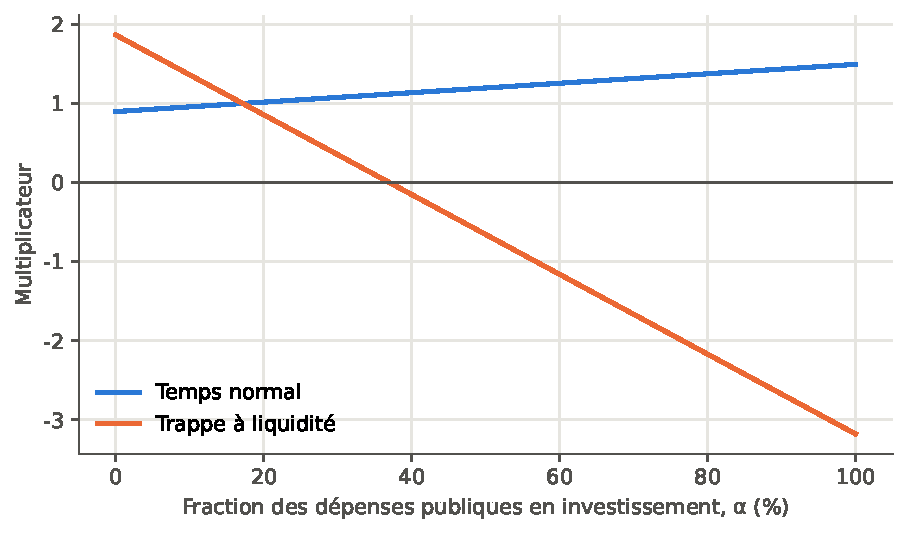
\includegraphics[width=0.8\textwidth]{figure_4_1}
\numfigure{4.1}{Multiplicateur en fonction de $\alpha$, financement du plan de relance par taxe forfaitaire}
\end{figure}

\begin{figure}[htbp]
\centering
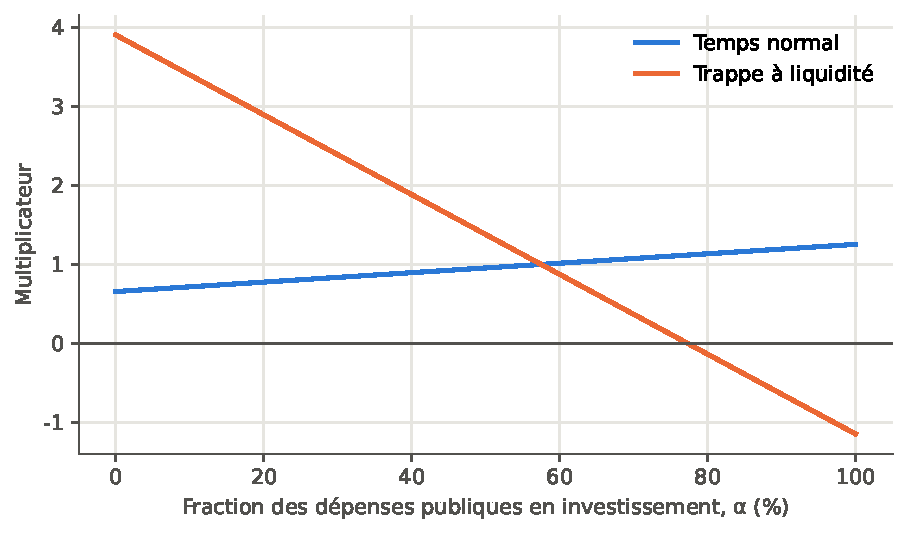
\includegraphics[width=0.8\textwidth]{figure_4_2}
\numfigure{4.2}{Multiplicateur en fonction de $\alpha$, financement du plan de relance par taxe sur le travail}
\end{figure}

\section{Cas général}

Les hypothèses simplificatrices selon lesquelles le capital public devient immédiatement productif et la dépréciation est complète s’avèrent peu réalistes, quand bien même les résultats précédents sont utiles pour comprendre l’intuition de l’impact de la trappe à liquidité et du type de financement sur le multiplicateur. Dans cette section, nous relâchons les hypothèses de la section précédente. En particulier, nous considérons un taux de dépréciation $\delta$ non nul et différents temps de construction du capital public, notamment $\T = 1$ et $\T = 16$.

Dans ce contexte plus général, nous générerons une trappe à liquidité en introduisant un choc sur la préférence pour la liquidité dans la fonction d’utilité des ménages. Ce choc a pour effet d’augmenter l’épargne des ménages dans les actifs sans risque. Afin de simplifier l’analyse, nous supposons que la fonction $F(.)$ est linéaire. Nous choisissons la taille du choc et sa persistance de sorte que la trappe à liquidité dure 12 trimestres. Le modèle est résolu à l’aide de Dynare en supposant qu’il n’y a pas d’incertitude (perfect foresight).

Étant donné que la dimension dynamique redevient importante dans la version générale du modèle, nous présenterons les multiplicateurs en valeur présente (\emph{MVP}), ce qui permet de mesurer la variation totale de la production dans le temps. Les MVP sont fréquemment utilisés dans la littérature et peuvent être présentés de la manière suivante :
\begin{align}
MVP &= \frac{\Et\sum_{t=0}^{h}(1+r_\beta)^{-t}(y_t - y)}{\Et\sum_{t=0}^{h}(1+r_\beta)^{-t}(g_t - g)} \quad \text{(temps normal)} \tag{55}\\
\intertext{et}
MVP &= \frac{\Et\sum_{t=0}^{h}(1+r_\beta)^{-t}\Delta y_t}{\Et\sum_{t=0}^{h}(1+r_\beta)^{-t}\Delta g_t} \quad \text{(trappe à liquidité)} \tag{56}
\end{align}
où $\Delta y_t$ et $\Delta g_t$ mesurent la différence entre le scénario avec un choc simultané sur les dépenses publiques et la préférence pour la liquidité et le scénario avec uniquement un choc sur la préférence pour la liquidité. Nous aborderons d’abord le cas où les dépenses du gouvernement sont uniquement financées par une taxe sur le revenu du travail. Dans la section suivante, nous introduisons la dette publique.

Nous maintenons la calibration décrite dans le tableau 4.1. Les paramètres additionnels sont calibrés comme suit : $\delta = 0.025$, $\phi_y = 0.05$, $\rho_\zeta = 0.95$ et $\rho_n = 0.5$ (voir Sims et Wolff, 2018).

\subsection{Modèle sans dette}

Dans cette sous-section, nous présentons les multiplicateurs à l’impact et actualisés sur 500 périodes pour les deux types de financement du plan de relance. Les tableaux 5.1 et 5.2 présentent ainsi les multiplicateurs en temps normal et en trappe à liquidité pour différents temps de construction du capital public. De plus, nous présentons ces multiplicateurs quand toutes les dépenses publiques sont destinées à l’investissement ($\alpha = 1$) et lorsqu’elles sont exclusivement destinées à la consommation ($\alpha = 0$).

\newcommand{\multtable}[9]{%
\begin{tabular}{llccc}
\toprule
& & $\alpha = 0$ & \multicolumn{2}{c}{$\alpha = 1$}\\
& & & $\T = 1$ & $\T = 16$\\
\midrule
\multirow{2}{*}{\textbf{Impact}} & Temps normal & #1 & #2 & #3\\
 & Trappe à liquidité & #4 & #5 & #6\\
\multirow{2}{*}{\textbf{\emph{MVP} sur 500 périodes}} & Temps normal & #7 & #8 & #9\\
}

\begin{table}[htbp]
\centering
\numtable{5.1}{Multiplicateurs à l’impact et en valeur présente, financement du plan de relance par taxe forfaitaire}
\multtable{0,8}{0,92}{0,76}{0,93}{0,95}{1,05}{0,8}{1,89}{1,80}
 & Trappe à liquidité & 0,93 & 1,88 & 2,20\\
\bottomrule
\end{tabular}
\end{table}

\begin{table}[htbp]
\centering
\numtable{5.2}{Multiplicateurs à l’impact et en valeur présente, financement du plan de relance par taxe sur le revenu du travail}
\multtable{0,55}{0,67}{0,51}{0,76}{0,75}{0,92}{0,54}{1,63}{1,55}
 & Trappe à liquidité & 0,84 & 1,76 & 2,11\\
\bottomrule
\end{tabular}
\end{table}

Intéressons-nous d’abord au cas $\alpha = 0$. En temps normal, lorsque le plan de relance est financé par une taxe forfaitaire (Tableau 5.1), on obtient un multiplicateur de 0,8 à l’impact et lorsqu’actualisé sur 500 périodes. Pour le financement par taxe sur le revenu du travail (Tableau 5.2), le multiplicateur est de 0,55 à l’impact et 0,54 lorsqu’actualisé sur 500 périodes.

Une hausse des dépenses publiques allouées à la consommation provoque une augmentation de la demande agrégée et donc de l’inflation. Ainsi, les autorités monétaires augmentent le taux d’intérêt nominal. Étant donné que la part des dépenses publiques destinées à l’investissement est nulle, le choc de dépenses n’a pas d’effet déflationniste qui permettrait de contrer l’augmentation de taux d’intérêt et donc de produire un multiplicateur budgétaire plus élevé.

En trappe à liquidité, lorsque le plan de relance est financé par une taxe forfaitaire (Tableau 5.1), le multiplicateur est de 0,93 à l’impact et lorsqu’actualisé sur 500 périodes. Pour le financement par taxe sur le revenu du travail (Tableau 5.2), le multiplicateur est de 0,76 à l’impact et 0,84 lorsqu’on l’actualise sur 500 périodes. La grande différence avec le contexte de temps normal est que le taux d’intérêt fixé par les autorités monétaires reste à zéro pendant plusieurs périodes. Ainsi, l’augmentation de l’inflation n’est plus contrebalancée par une augmentation du taux d’intérêt nominal. Par voie de conséquence, le taux d’intérêt réel baisse et la production est plus stimulée qu’en temps normal, ce qui explique que les multiplicateurs soient plus élevés.

Étant donné que les dépenses publiques du plan de relance ne sont pas destinées au capital public, les ménages n’anticipent pas de gain de productivité et donc de richesse, cela limite ainsi la hausse de la consommation et donc le multiplicateur. C’est la raison pour laquelle les multiplicateurs sont plus élevés lorsque $\alpha$ est non nul et qu’il y a un délai de construction du capital.

\begin{figure}[htbp]
\centering
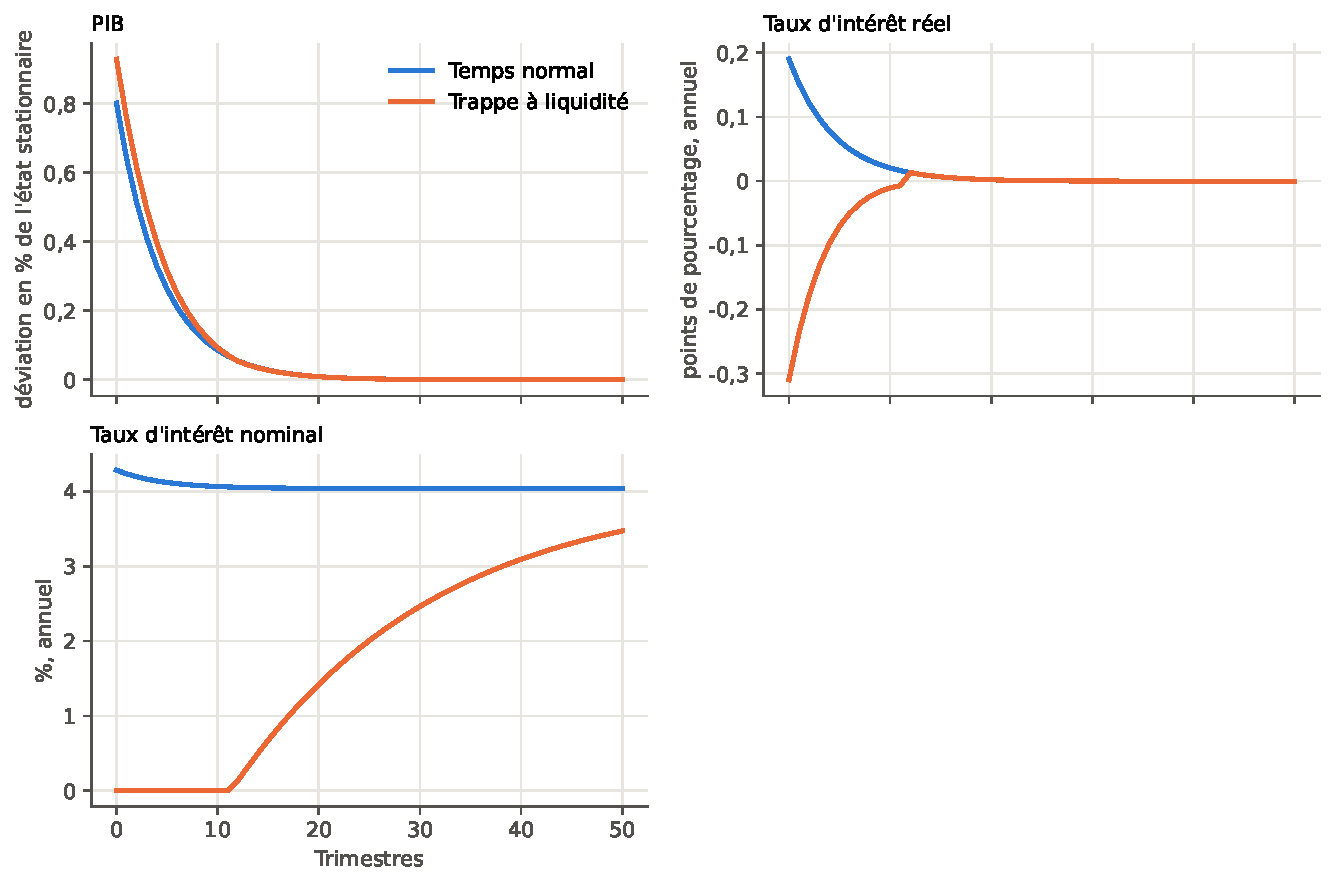
\includegraphics[width=\textwidth]{figure_5_1}
\numfigure{5.1}{Fonctions de réponse à un choc de dépenses publiques lorsque $\alpha = 0$, financement par taxe forfaitaire}
\end{figure}

\begin{figure}[htbp]
\centering
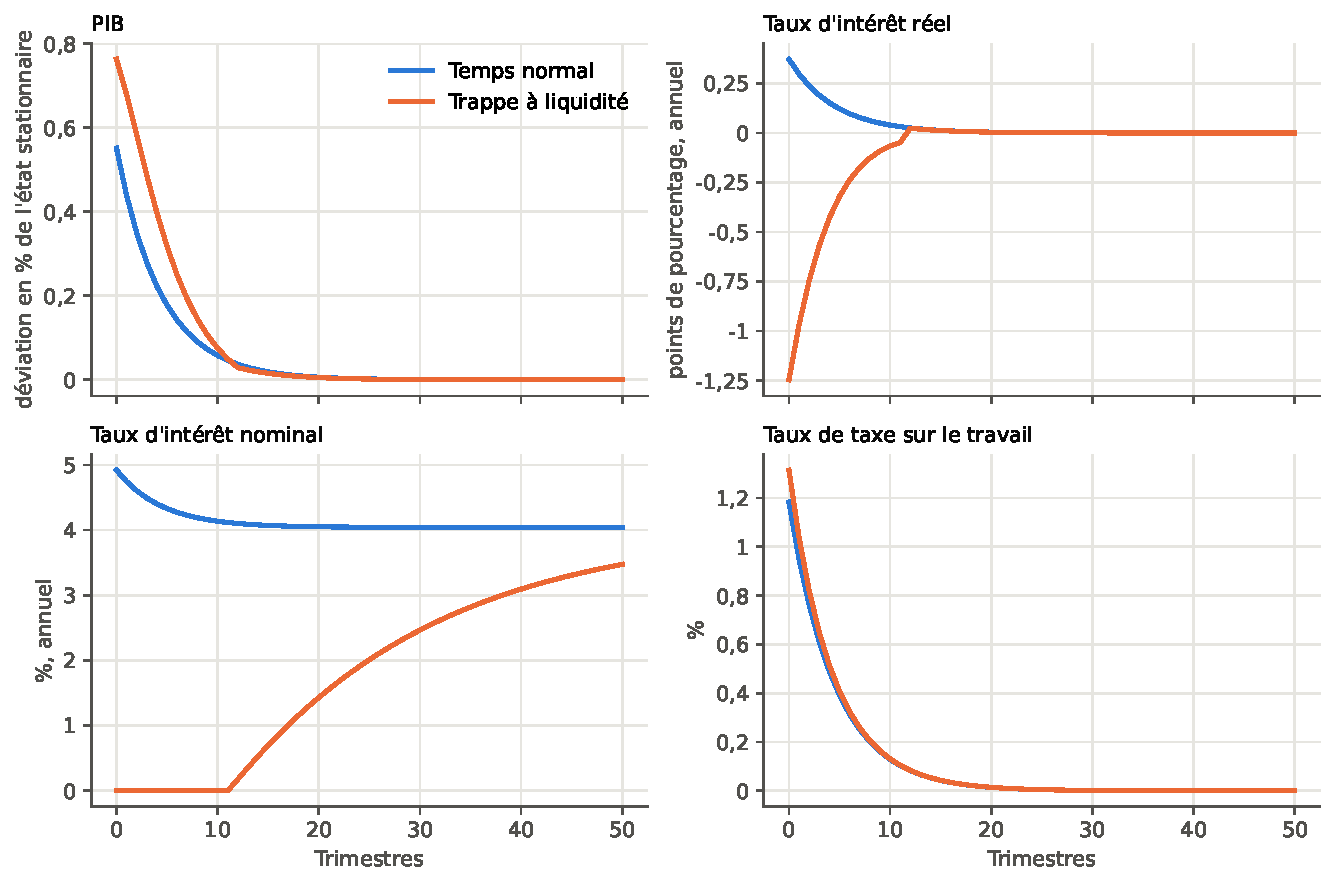
\includegraphics[width=\textwidth]{figure_5_2}
\numfigure{5.2}{Fonctions de réponse à un choc de dépenses publiques lorsque $\alpha = 0$, financement par taxe sur le travail}
\end{figure}

En temps normal, et lorsque le plan de relance est financé par une taxe sur le revenu du travail (Graphique 5.2), le taux d’intérêt réel augmente plus qu’avec un financement par taxe forfaitaire (Graphique 5.1). Alors, dans le cas du financement par taxe sur le revenu du travail, les multiplicateurs sont moins élevés.

En trappe à liquidité, on remarque que pour le cas du financement par taxe sur le revenu du travail, le taux d’intérêt réel baisse beaucoup plus que pour le financement par taxe forfaitaire, étant donné l’effet inflationniste de la taxe sur le revenu du travail qui, rappelons-le, est une taxe distorsive. Cela explique pourquoi la différence entre le multiplicateur en trappe et en temps normal est plus grande pour le financement par taxe sur le revenu du travail. Les multiplicateurs correspondant au financement par taxe forfaitaire sont malgré tout plus grands en trappe que pour le cas du financement par taxe sur le revenu du travail.

Analysons maintenant le cas où $\alpha = 1$ et où le temps de construction du capital est de 1 trimestre. En temps normal, lorsque le plan de relance est financé par une taxe forfaitaire (Tableau 5.1), on obtient un multiplicateur de 0,92 à l’impact et de 1,89 pour la valeur actualisée sur 500 périodes. Pour le financement par taxe sur le revenu du travail (Tableau 5.2), le multiplicateur est de 0,67 à l’impact et de 1,63 lorsqu’actualisé sur 500 périodes. Les multiplicateurs sont plus élevés que dans le cas précédent.

Étant donné que toutes les dépenses publiques du plan de relance sont destinées à l’investissement dans le capital, le choc de dépenses va avoir comme effet de baisser les coûts marginaux, ce qui exerce une pression déflationniste. Cet effet arrive relativement vite étant donné que le temps de construction n’est que d’un trimestre. Ainsi, l’augmentation du taux d’intérêt nominal décrite dans le cas précédent est largement amoindrie, ce qui a un effet positif sur la production.

En trappe à liquidité, lorsque le plan de relance est financé par une taxe forfaitaire (Tableau 5.1), le multiplicateur est de 0,95 à l’impact et de 1,88 lorsqu’on l’actualise sur 500 périodes. Pour le financement par taxe sur le revenu du travail (Tableau 5.2), le multiplicateur est de 0,75 à l’impact et de 1,76 lorsqu’on l’actualise sur 500 périodes.

L’intuition derrière le fait que le multiplicateur en trappe est plus élevé qu’en temps normal reste similaire à ce qui a été déjà décrit précédemment. En trappe à liquidité, toute pression inflationniste pousse le multiplicateur vers le haut. Étant donné la construction de capital public, les ménages anticipent des gains de productivité et donc de richesse. C’est d’autant plus le cas que le temps de construction est long, c’est pourquoi lorsque le temps de construction est trop court, il n’est pas impossible d’observer un multiplicateur plus bas en trappe qu’en temps normal.

\begin{figure}[htbp]
\centering
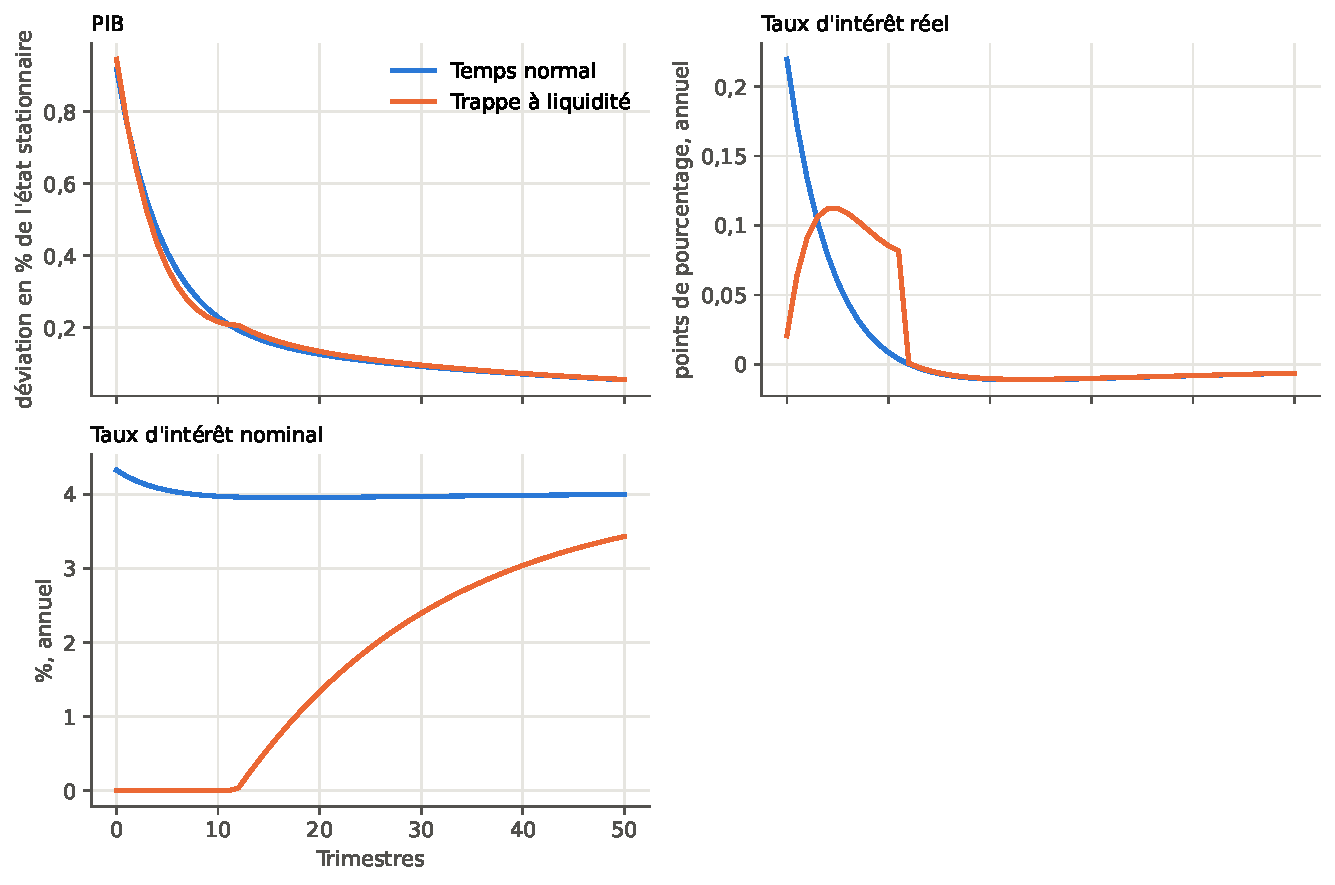
\includegraphics[width=\textwidth]{figure_5_3}
\numfigure{5.3}{Fonctions de réponse à un choc d’investissement public lorsque $\alpha = 1$ et $\T = 1$, financement par taxe forfaitaire}
\end{figure}

\begin{figure}[htbp]
\centering
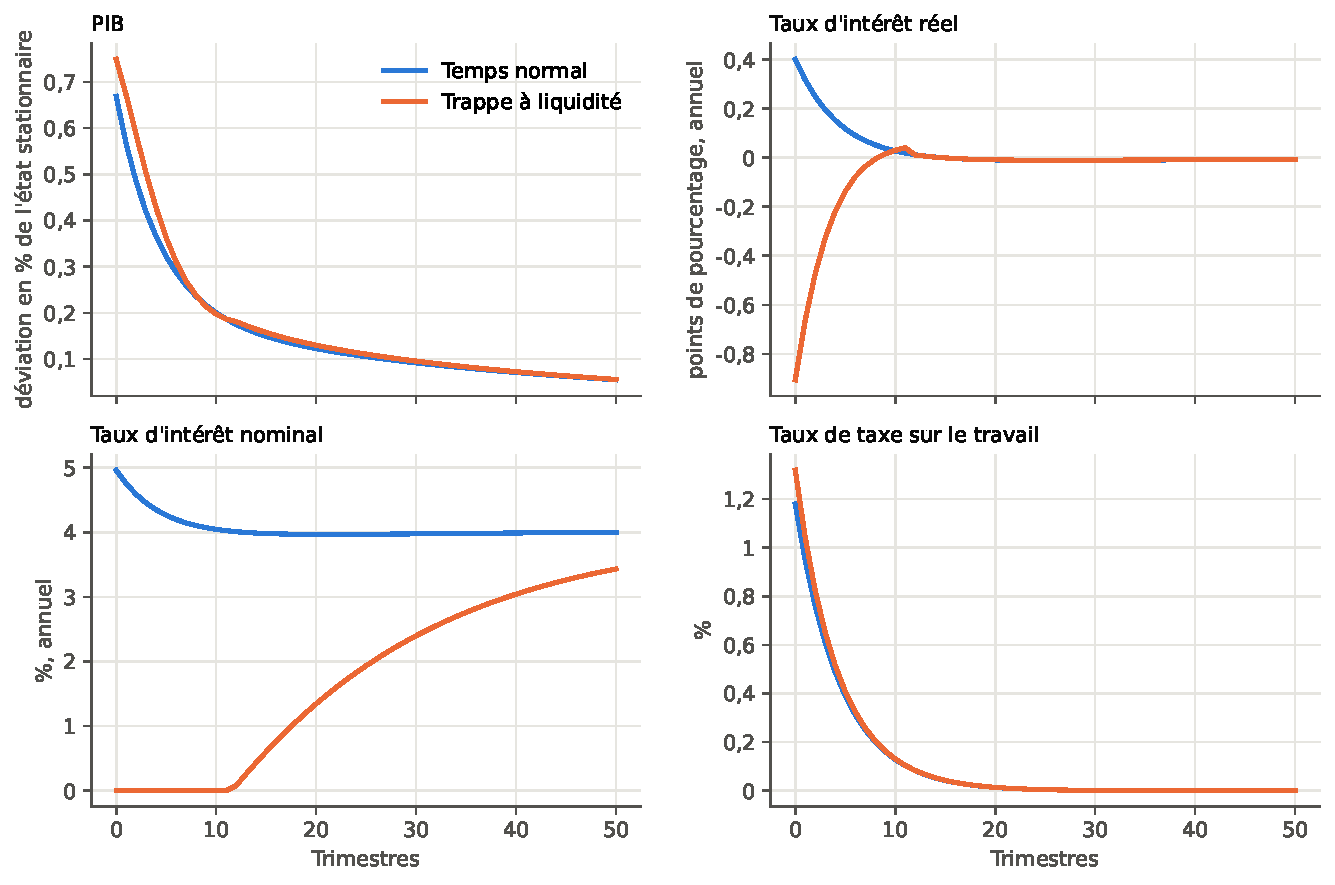
\includegraphics[width=\textwidth]{figure_5_4}
\numfigure{5.4}{Fonctions de réponse à un choc d’investissement public lorsque $\alpha = 1$ et $\T = 1$, financement par taxe sur le travail}
\end{figure}

Pour le financement par taxe forfaitaire (Graphique 5.3), les pressions inflationnistes ne sont pas assez fortes pour faire chuter initialement le taux d’intérêt réel lorsque le temps de construction du capital est de 1 trimestre. En revanche, dans le cas du financement par taxe sur le revenu du travail (Graphique 5.4), il y a beaucoup plus de pressions inflationnistes étant donné la taxe sur le revenu du travail, alors le multiplicateur en trappe est plus élevé qu’en temps normal. Cependant, les multiplicateurs pour le financement forfaitaire sont plus élevés qu’avec un financement par taxe sur le revenu du travail en vertu de la baisse persistante du taux d’intérêt réel à la sortie de la trappe dans le premier cas.

Analysons maintenant le cas où $\alpha = 1$ et où le temps de construction du capital est de 16 trimestres. En temps normal, lorsque le plan de relance est financé par une taxe forfaitaire (Tableau 5.1), on obtient un multiplicateur de 0,76 à l’impact et de 1,80 pour la valeur actualisée sur 500 périodes. Pour le financement par taxe sur le revenu du travail (Tableau 5.2), le multiplicateur est de 0,51 à l’impact et de 1,55 lorsqu’actualisé sur 500 périodes. En trappe à liquidité, lorsque le plan de relance est financé par une taxe forfaitaire (Tableau 5.1), le multiplicateur est de 1,05 à l’impact et de 2,20 lorsqu’on l’actualise sur 500 périodes. Pour le financement par taxe sur le revenu du travail (Tableau 5.2), le multiplicateur est de 0,92 à l’impact et de 2,11 lorsqu’on l’actualise sur 500 périodes.

Il est intéressant d’observer que lorsque le temps de construction est plus long, en l’occurrence 16 trimestres, le multiplicateur budgétaire tend à baisser en temps normal alors qu’il augmente en trappe à liquidité. Effectivement, lorsque le temps de construction est long, les gains de productivité anticipés par les agents surviennent très loin dans le futur, et donc n’ont pas autant d’effet sur la demande agrégée actuelle, réduisant ainsi le multiplicateur budgétaire en temps normal. En trappe à liquidité, cet effet est plus que compensé par le retardement de l’effet désinflationniste résultant de la baisse du coût marginal futur, ce qui amplifie le multiplicateur.

\begin{figure}[htbp]
\centering
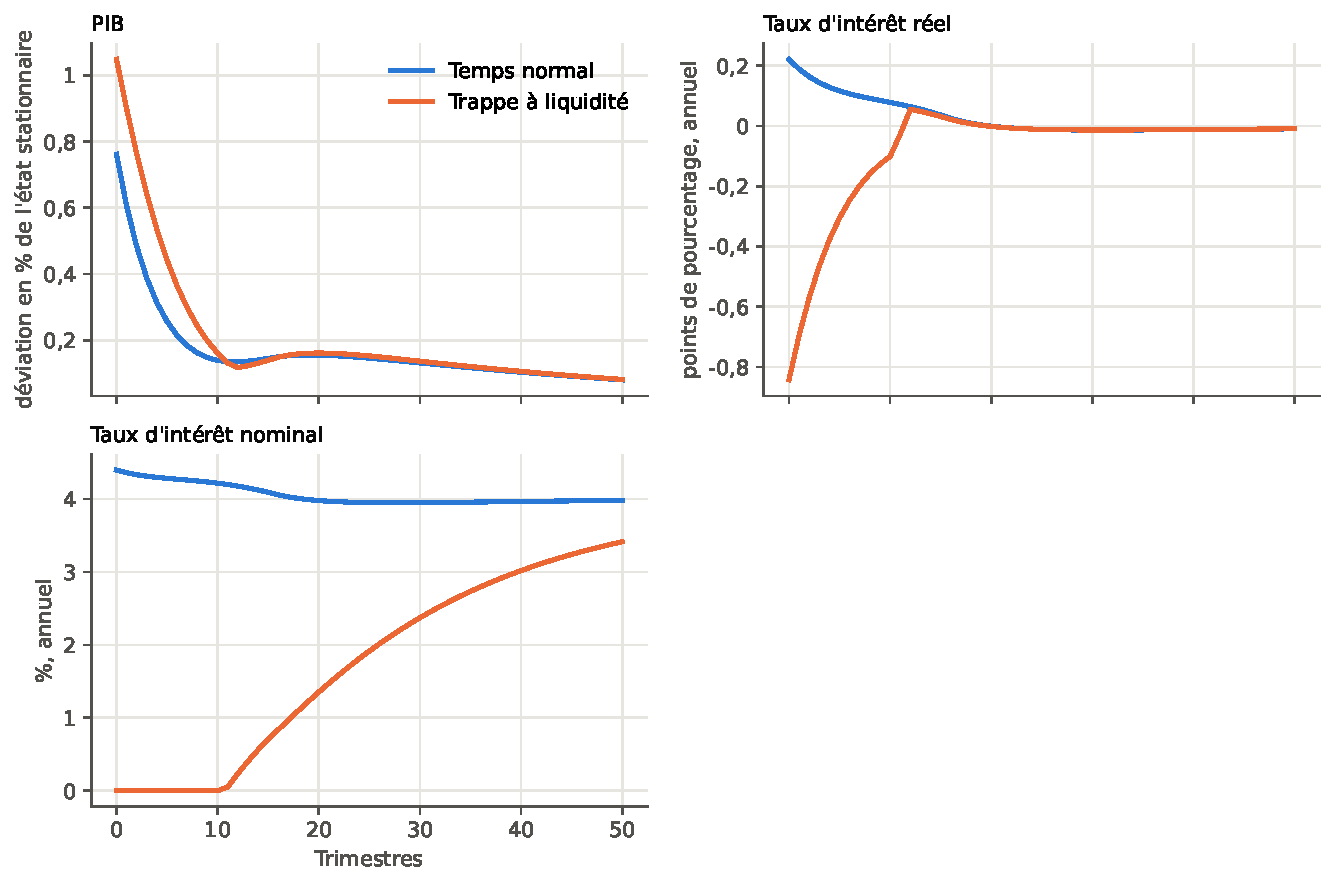
\includegraphics[width=\textwidth]{figure_5_5}
\numfigure{5.5}{Fonctions de réponse à un choc d’investissement public lorsque $\alpha = 1$ et $\T = 16$, financement forfaitaire}
\end{figure}

\begin{figure}[htbp]
\centering
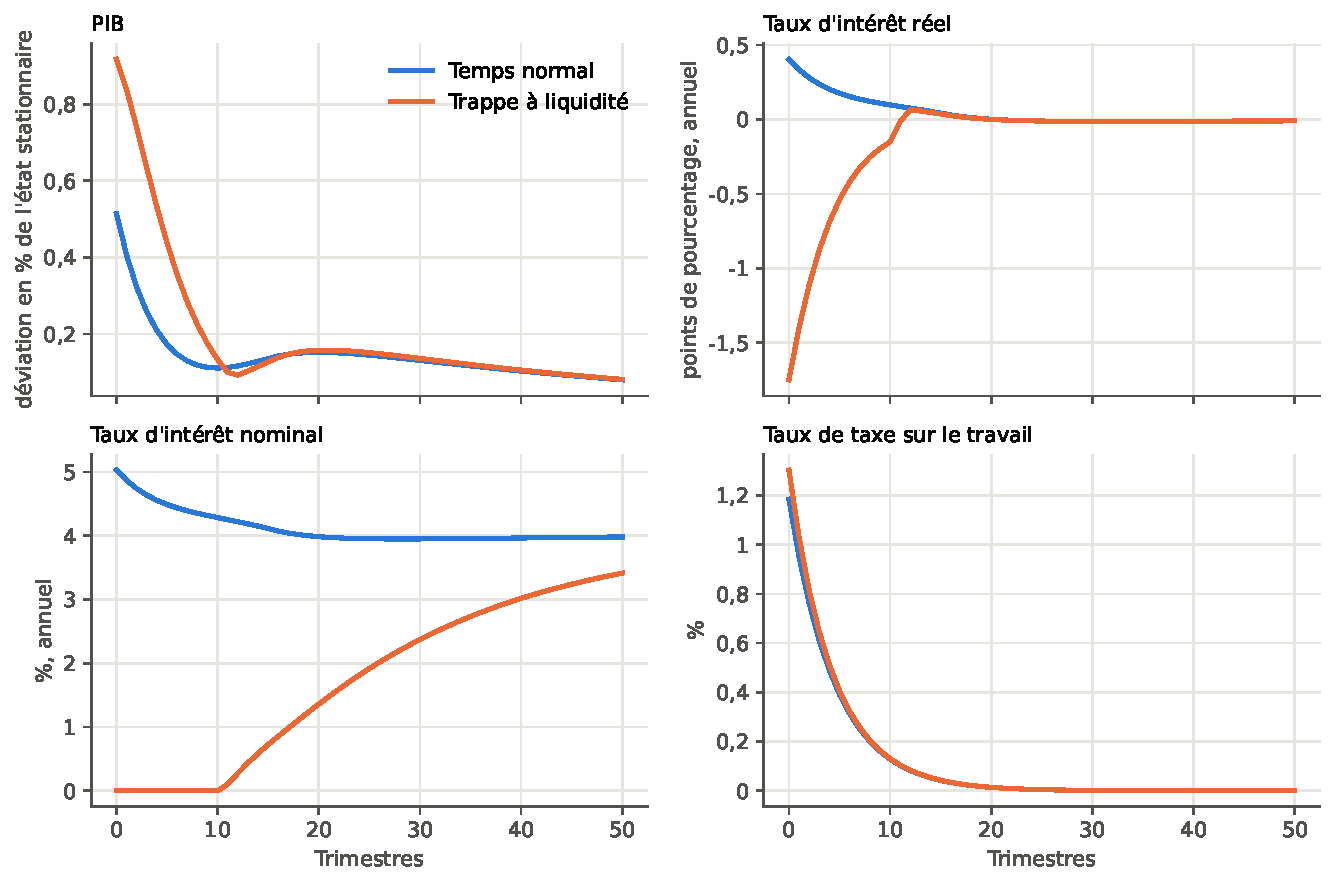
\includegraphics[width=\textwidth]{figure_5_6}
\numfigure{5.6}{Fonctions de réponse à un choc d’investissement public lorsque $\alpha = 1$ et $\T = 16$, financement par taxe sur le travail}
\end{figure}

Un élément qui reste à être discuté dans cette section est le fait que les multiplicateurs dans le cas du financement par taxe forfaitaire sont plus élevés que dans le cas du financement par taxe sur le revenu du travail en trappe à liquidité, peu importe la part des dépenses destinées au capital et le temps de construction. Cela semble alors être contradictoire avec ce que nous avions trouvé lors de la résolution algébrique. Cela peut s’expliquer par le processus de la taxe sur le revenu du travail qui diffère par rapport au cas de la résolution du modèle linéaire. Lors de la résolution algébrique, nous avions considéré un processus markovien sur $\beta_t$ pour générer la trappe à liquidité. Cela avait pour conséquence qu’en sortie de trappe, toutes les variables du modèle revenaient immédiatement à leur état stationnaire, y compris la taxe sur le revenu du travail, puisque cette version du modèle n’avait pas de variable d’état endogène. Tel n’est pas le cas dans la version générale du modèle où la sortie de trappe est endogène. En effet, après un choc sur la préférence pour la liquidité, la taxe sur le revenu du travail demeure plus élevée que son niveau initial (nul) même lorsque l’économie est sortie de trappe, et ne revient vers celui-ci que très progressivement (voir Graphiques 5.2, 5.4 et 5.6). Les agents anticipent donc une baisse de leur revenu futur après impôt relativement à une situation où la taxe serait nulle, ce qui affecte négativement le multiplicateur budgétaire.

La trajectoire de la taxe sur le revenu du travail est donc déterminante pour la taille du multiplicateur. Dans la prochaine section, avec l’ajout de la dette, nous serons en mesure d’apporter plus d’éclairage sur cette question.

\subsection{Modèle avec dette}

Nous arrivons à la version la plus élaborée de notre modèle, celle où les dépenses du gouvernement sont financées par une taxe forfaitaire, une taxe sur le revenu du travail et la dette. Rappelons que la taxe sur le revenu du travail s’ajuste à la dette passée selon un processus inspiré de Sims et Wolff (2018) :
\begin{equation*}
\tau_t = (1-\rho_n)\tau + \rho_n\tau_{t-1} + (1-\rho_n)\gamma_n\left(\frac{B_{t-1}}{Y_t} - \frac{B}{Y}\right)
\end{equation*}
qui a déjà été décrit dans la section 3. Nous choisissons $\gamma_n$ tel que le ratio dette sur PIB ne soit pas explosif. Nous fixons $\gamma_n = 0.1$ et $\rho_n = 0.5$ comme Sims et Wolff (2018). C’est à travers le paramètre $\gamma_n$ que nous pouvons ajuster la trajectoire de la taxe en trappe à liquidité, il sera donc intéressant de faire une analyse de sensibilité sur ce paramètre. Comme fait précédemment, nous calculerons le multiplicateur budgétaire en temps normal, en trappe à liquidité et pour différents temps de construction du capital public. Nous considérons uniquement le cas où la taxe et la dette sont nulles à l’état stationnaire, pour être en mesure de faire une comparaison avec les multiplicateurs obtenus précédemment.

\begin{table}[htbp]
\centering
\numtable{6.1}{Multiplicateurs avec financement par dette et $\gamma_n = 0.1$}
\multtable{0,63}{0,75}{0,59}{0,98}{0,99}{1,10}{0,07}{1,16}{1,07}
 & Trappe à liquidité & 0,57 & 1,54 & 1,81\\
\bottomrule
\end{tabular}
\end{table}

Les multiplicateurs à l’impact en temps normal chutent par rapport au cas du financement exclusif par taxe sur le revenu du travail. En revanche, en trappe à liquidité, les multiplicateurs sont plus grands. Cela suggère qu’il soit possible de réconcilier nos résultats avec ceux obtenus algébriquement en faisant varier $\gamma_n$ qui joue un rôle déterminant sur la trajectoire de la taxe. Nous réalisons donc une analyse de sensibilité sur le paramètre $\gamma_n$ lorsque $\alpha = 1$ et que le temps de construction du capital public est de 16 trimestres. Puisque les valeurs considérées doivent rester cohérentes avec les estimations de la littérature, nous faisons varier $\gamma_n$ dans l’intervalle [0,05 ; 0,25].

\begin{figure}[htbp]
\centering
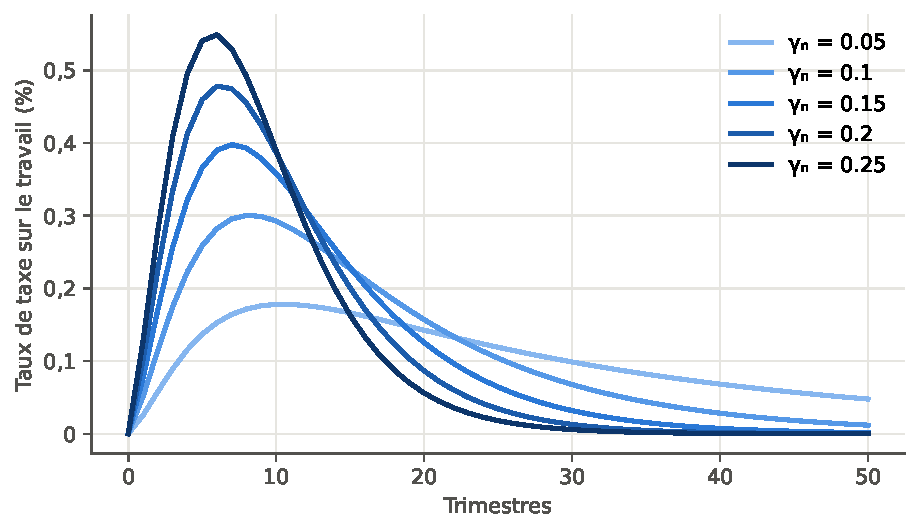
\includegraphics[width=0.8\textwidth]{figure_6_1}
\numfigure{6.1}{Trajectoire de la taxe sur le revenu du travail en fonction de $\gamma_n$ en trappe à liquidité lors d’un choc des dépenses publiques}
\end{figure}

\begin{table}[htbp]
\centering
\numtable{6.2}{Multiplicateurs en trappe à liquidité lorsque $\T = 16$}
\begin{tabular}{ccc}
\toprule
$\gamma_n$ & Multiplicateur à l’impact & MVP sur 500 périodes\\
\midrule
0,05 & 1,05 & 1,65\\
0,1 & 1,10 & 1,81\\
0,15 & 1,15 & 1,96\\
0,2 & 1,18 & 2,08\\
0,25 & 1,20 & 2,15\\
\bottomrule
\end{tabular}
\end{table}

On remarque ainsi que plus $\gamma_n$ est élevé, moins la taxe est persistante et plus elle monte à des niveaux élevés en trappe (voir Graphique 6.1), augmentant ainsi la valeur du multiplicateur. Il existerait donc un niveau de $\gamma_n$ qui assurerait un compromis entre niveau et persistance de la taxe en trappe à liquidité de sorte que le multiplicateur budgétaire soit plus élevé qu’avec financement par taxe forfaitaire. À l’impact, ceci est le cas dès que $\gamma_n$ dépasse le seuil de 0,05. Pour le MVP, la valeur minimale requise de $\gamma_n$ est légèrement supérieure à la borne maximale considérée (0,25).

\section{Conclusion}

Dans ce mémoire, nous avons comparé le multiplicateur budgétaire à travers différents types de financement d’un plan de relance au sein d’un même modèle ayant un état stationnaire unique. Le fait de faire varier le type de financement des dépenses publiques uniquement hors de l’état stationnaire nous a permis de faire une comparaison analytique des multiplicateurs en temps normal et en trappe à liquidité en considérant un modèle linéaire statique et ensuite de déterminer si, et dans quel contexte, les résultats analytiques tiennent dans un modèle non linéaire dynamique.

Nos résultats ont permis de mettre en évidence l’importance du mode de financement quant à la taille du multiplicateur. Notre conclusion principale est que, dans la mesure où la hausse de l’impôt sur le revenu du travail a lieu principalement pendant que l’économie est en trappe à liquidité mais qu’elle se résorbe aussitôt que l’économie est sortie de trappe, il est possible d’avoir un multiplicateur budgétaire comparable (et potentiellement supérieur) à celui correspondant à un financement par taxe forfaitaire.

Maintenant, il serait intéressant dans de futures recherches d’étendre le modèle présenté dans ce mémoire pour tenir compte d’autres types de taxes distorsives telles que la taxe sur la consommation ou encore l’impôt sur le revenu du capital. Également, pour compléter la littérature, il serait pertinent de déterminer la politique budgétaire optimale dans une économie qui dispose de plusieurs instruments fiscaux mais dans laquelle le gouvernement est contraint de suivre des règles fiscales préétablies.

\newpage
\section*{Bibliographie}
\addcontentsline{toc}{section}{Bibliographie}
\begin{list}{}{\setlength{\leftmargin}{2em}\setlength{\itemindent}{-2em}\setlength{\itemsep}{0.3em}}
\small
\item Aloui, R. et A. Eyquem (2019). « Spending multipliers with distortionary taxes: Does the level of public debt matter? », \emph{Journal of Macroeconomics}, vol. 60, p. 275-293.
\item Altig, D., L. J. Christiano, M. Eichenbaum et J. Linde (2011). « Firm-specific capital, nominal rigidities and the business cycle », \emph{Review of Economic Dynamics}, vol. 14, no 2, p. 225-247.
\item Auerbach, Alan, J et Yuriy Gorodnichenko (2012). « Measuring the output responses to fiscal policy », \emph{American Economic Journal: Economic Policy}, vol. 4, p. 1-27.
\item Barro, Robert J (1974). « Are government bonds net wealth? », \emph{J.P.E}, vol. 82, p. 1095-1117.
\item Bom, P. R. D. et J. E. Ligthart (2014). « What have we learned from three decades of research on the productivity of public capital? », \emph{Journal of Economic Surveys}, vol. 28, no 5, p. 889-916.
\item Boehm, C. (2020). « Government consumption and investment: Does the composition of purchases affect the multiplier? », \emph{Journal of Monetary Economics}, vol. 115, p. 80-93.
\item Bouakez, H., M. Guillard et J. Roulleau-Pasdeloup (2017). « Public investment, time to build, and the zero lower bound », \emph{Review of Economic Dynamics}, vol. 23, p. 60-79.
\item Bouakez, H., M. Guillard et J. Roulleau-Pasdeloup (2020). « The optimal composition of public spending in a deep recession », \emph{Journal of Monetary Economics}, vol. 114, p. 330-349.
\item Bouakez, H., F. Larocque et M. Normandin (2018). « Separating the wheat from the chaff: A disaggregate analysis of the effects of public spending in the US », \emph{Canadian Journal of Economics}, vol. 51, no 2, p. 361-390.
\item Christiano, L., M. Eichenbaum et S. Rebelo (2011). « When is the government spending multiplier large? », \emph{Journal of Political Economy}, vol. 119, no 1, p. 78-121.
\item Eggertsson, G. B. (2011). « What fiscal policy is effective at zero interest rates? », \emph{NBER Macroeconomics Annual}, vol. 25.
\item Jord\`a, \`O. (2005). « Estimation et Inference of Impulse Responses by Local Projections », \emph{American Economic Review}, vol. 95, no 1, p. 161-182.
\item Keynes (1936). \emph{The general theory of employment interest and money}.
\item Kydland, F. E. et E. C. Prescott (1982). « Time to build and aggregate fluctuations », \emph{Econometrica}, vol. 50, no 6, p. 1345-1370.
\item Lemoine, M. et J. Lind\'e (2023). « Fiscal stimulus in liquidity traps: Conventional or unconventional policies? », \emph{European Economic Review}, vol. 151.
\item Lucas, R. E. (1976). « Econometric policy evaluation - critique », \emph{Carnegie-Rochester Conference Series on Public Policy}, vol. 1, p. 19-46.
\item Miyamoto, W., TL. Nguyen et D. Sergeyev (2018). « Government spending multipliers under the zero lower bound: Evidence from japan. », \emph{American Economic Journal-Macroeconomics}, vol. 10, no 3.
\item Nakata, Taisuke (2017). « Optimal government spending at the zero lower bound: A non-ricardian analysis », \emph{Review of Economic Dynamics}, vol. 23, p. 150-169.
\item Perotti, R (2004). « Public Investment: Another (Different) Look », IGIER, Working Paper no 277, p. 49.
\item Ramey, V. A. (2019). « Ten years after the financial crisis: What have we learned from the renaissance in fiscal research? », \emph{Journal of Economic Perspectives}, vol. 33, no 2, p. 89-114.
\item Ramey, V. A. (2020). « The macroeconomic consequences of infrastructure investment », National Bureau of Economic Research.
\item Ramey, V. A. et S. Zubairy (2018). « Government spending multipliers in good times and in bad: Evidence from us historical data », \emph{Journal of Political Economy}, vol. 126, no 2, p. 850-901.
\item Sims, E et J. Wolff (2018). « The output and welfare effects of government spending shocks over the business cycle », \emph{International Economic Review}, vol. 59, no 3, p. 1403-1435.
\item Woodford, M. (2011). « Simple analytics of the government expenditure multiplier », \emph{American Economic Journal-Macroeconomics}, vol. 3, no 1, p. 1-35.
\end{list}

\newpage
\appendix
\section*{Annexe A : État stationnaire}
\addcontentsline{toc}{section}{Annexe A : État stationnaire}

Pour résoudre l’état stationnaire, nous nous servirons de deux identités particulièrement utiles
\begin{equation}
\frac{Y}{C} = \frac{1}{1-\gbar} \tag{1}
\end{equation}
et
\begin{equation}
G = \frac{\gbar}{1-\gbar}C \tag{2}
\end{equation}

\subsection*{Coût marginal}

On peut calculer l’état stationnaire du coût marginal à partir de la condition de premier ordre des producteurs des biens intermédiaires
\begin{equation*}
MC = \frac{\theta-1}{\theta} + \frac{\XX}{\theta}\pi(1+\pi) - \frac{\XX}{\theta}\frac{U_c}{U_c}\frac{Y}{Y}\pi(1+\pi)
\end{equation*}
Étant donné que l’inflation est nulle à l’état stationnaire, on obtient facilement le coût marginal à l’état stationnaire :
\begin{equation*}
\boldsymbol{MC = \frac{\theta-1}{\theta}}
\end{equation*}

\subsection*{Travail}

On peut calculer le travail à l’état stationnaire en utilisant les équations d’offre et de demande :
\begin{align*}
w &= \frac{-U_N}{U_C(1-\tau)}\\
w &= MC.F_N
\end{align*}
où $\frac{-U_N}{U_C} = \frac{1-\gamma}{1-N}\frac{C}{\gamma}$ et $F_N = a\frac{F}{N}$. On a donc
\begin{equation*}
\frac{1}{(1-\tau)}\frac{1-\gamma}{1-N}\frac{C}{\gamma} = aMC\frac{F}{N}
\end{equation*}
En remplaçant $MC$ par $\frac{\theta-1}{\theta}$ et en utilisant le fait que $\frac{F}{C} = \frac{Y}{C} = \frac{1}{1-\gbar}$, on peut isoler $N$ et l’exprimer en fonction des paramètres du modèle :
\begin{equation*}
\boldsymbol{N = \left(\frac{1-\gamma}{\gamma}\frac{1}{1-\tau}\frac{1-\gbar}{a}\frac{\theta}{\theta-1} + 1\right)^{-1}}
\end{equation*}

\subsection*{Consommation}

Grâce à la loi d’accumulation du capital, l’équation (19), on peut définir
\begin{equation*}
\delta K = G^i = \abar G
\end{equation*}
On a donc
\begin{equation*}
K = \frac{\abar}{\delta}G
\end{equation*}
En utilisant l’identité (2) on a :
\begin{equation*}
K = \frac{\abar\gbar}{\delta(1-\gbar)}C
\end{equation*}
De plus, on a :
\begin{equation*}
Y = N^a K^b
\end{equation*}
En utilisant l’identité (1), on peut exprimer $C$ en fonction de $N$ et $K$ :
\begin{equation*}
C = (1-\gbar)N^a K^b
\end{equation*}
Maintenant, en exprimant $K$ en fonction de $C$, on peut exprimer $C$ en fonction de $N$ et des paramètres du modèle :
\begin{equation*}
\boldsymbol{C = \left((1-\gbar)N^a\left(\frac{\abar\gbar}{\delta(1-\gbar)}\right)^b\right)^{\frac{1}{1-b}}}
\end{equation*}
À partir de là, il suffit de substituer les valeurs de $N$ et de $C$ dans les équations qui les contiennent pour obtenir :
\begin{align*}
\boldsymbol{K} &\boldsymbol{= \frac{\abar\gbar}{\delta(1-\gbar)}C}\\
\boldsymbol{G} &\boldsymbol{= \frac{\delta K}{\abar}}\\
\boldsymbol{W} &\boldsymbol{= \frac{1-\gamma}{\gamma}\frac{C}{1-N}\frac{1}{1-\tau}}\\
\boldsymbol{Y} &\boldsymbol{= C+G}
\end{align*}

\subsection*{Taux d’intérêt nominal}

À l’instar de la littérature, on fixe le taux d’intérêt nominal de la manière suivante :
\begin{equation*}
\boldsymbol{i = \frac{1}{\beta} - 1}
\end{equation*}

\subsection*{Taxe sur le revenu du travail}

Pour avoir un seul et même état stationnaire dans tous les cas de figure, on fixe la taxe sur le revenu du travail à zéro.
\begin{equation*}
\boldsymbol{\tau = 0}
\end{equation*}

\subsection*{Dette}

À l’état stationnaire on a :
\begin{equation*}
G + iB \leq T + \tau WN
\end{equation*}
On sait également qu’à l’état stationnaire $T = G$ pour avoir le même état stationnaire que dans le financement du plan de relance par taxe forfaitaire. Alors on a :
\begin{equation*}
\boldsymbol{\frac{B}{P} = \frac{\tau WN}{i} = 0}
\end{equation*}
où $i = \frac{1}{\beta} - 1$.

\newpage
\section*{Annexe B : codes Dynare}
\addcontentsline{toc}{section}{Annexe B : codes Dynare}

\subsection*{Cas sans dette}
\lstinputlisting{annex_b_nodebt_fr.mod}

\subsection*{Cas avec dette}
\lstinputlisting{annex_b_debt_fr.mod}

\end{document}
